%- princip je využití atributů
%- kernely a kus z related work
% algoritmus
%- vlastnosti - věty o metrikách - možná zvláštni kapitola

\chapter{Attribute Assignment}
\label{chapter:attributeAssignment}
In Chapter \ref{chapter:preliminaries}, we defined the problem of metalearning, particularly the problem of algorithm selection and ranking. We have presented a general workflow that -- given some distance measure between attributes and a new dataset -- can rank algorithms based on previous experience. We also presented a distance measure based on the vector of global metadata. We have shown that this distance measure can be a metric on the space of datasets if the distance between the vector of global metafeatures is a metric. The room for improvement lies in the fact that for each dataset with arbitrary number of attributes, rows, and attribute domains, the number of global metadata extracted is always the same for each dataset. The ability to deal with such unstructured data has been recognized as a difficult and important task \cite{BrazdilMetalearning-2009,RepresentationalIssuesInMetalearning}. 

The main contribution of this thesis lies in the proposal and analysis of algorithms that can handle non-propositional representation of datasets without losing information that can occur when extracting fixed amount information from the common structure of the datasets. We start by discussing the importance of dealing with unstructured data and by presenting unstructured domains and algorithms that are able to tackle associated issues. Namely, we will discuss vector embeddings on the space of strings together with kernel methods on arbitrary spaces. We will explain why such techniques cannot be applied directly to the space of datasets. We will review recent attempts of how to handle non-propositional representations in the metalearning domain. Finally, we propose concept of attribute assignment given some attribute distance measure. If the datasets have different number of attributes, dummy attributes are added to the dataset with less attributes. Dataset distance is computed based on sum of attribute distances given by the assignment. We will present several algorithms derived from this concept. The first supports only simple attribute distance measures but can be computed quickly. The second is based on the Hungarian algorithm and can handle arbitrary attribute distance measure. We will present some examples to give the reader a clear idea about the algorithms. 

Then, theoretical properties of the proposed algorithms are discussed. It turns out that if the distance on the space of attributes extended by the dummy attribute is a metric then the resulting distance measure between datasets must also be a metric. We will also show that the same holds for the other direction. Yet we will discuss that the former direction is somewhat stronger if we only care about a metric on some subsets of dataset and attribute space. This can be useful if we optimize metric properties on some training data. These theorems also mean that we can use attribute metrics based on $p$-norms and their weighted counterparts and we get a metric on dataset space as well. We will discuss conditions that are necessary for the resulting dataset distance to be a metric. We will especially discuss the addition of dummy attribute followed by the discussion on what is the best way how to add such dummy attributes into the attribute distance. We also show that if we normalized the resulting dataset distance by the number of attributes, we could break the metric properties.

\section{Dealing with Unstructured Data}
During last decades, many machine learning and data mining techniques emerged. Almost all of them were designed to handle propositional data, usually encoded as a vector of fixed size.
However, not all data have this nice structure and there are lots of real world problems that are defined on unstructured data. \emph{Natural language processing} (NLP) tasks are defined on the space of strings (words and texts) and many traditional methods are  therefore not applicable. Another example of such unstructured space is the space of graphs. Many things such us social network connections can be naturally described using graphs. Therefore, it is important to investigate means of modifying machine learning tools to handle various non-propositional representations.
In this section, we shall present two notable approaches to deal with unstructured data.


\subsection{Word Embeddings}
Word embeddings is the set of natural language processing techniques where words or phrases are mapped to the real-valued vectors.
A well known example of word embedding is \emph{word2vec} \cite{word2vec,mikolovDistirbutedRepresentationsOfWords}.
Word2vec uses two different types of models to learn the vectors. The first one -- \emph{Continuous Bag-of-Word Model} or CBOW -- tries to predict the target word given the surrounding words (so called context). The CBOW uses the probabilistic feedforward neural network \cite{BengioNeuralProbabilisticLanguageModel} to  estimate the probabilities of current word. The desired vector is the weight vector between the hidden layer and the neuron in the output neuron corresponding to the word in question. The \emph{Skip-Gram Model} is the opposite of CBOW. The goal now is to guess the context given the word in the middle. 

The interesting part is that the trained vectors capture many linguistic regularities \cite{MikolovLinguisticRegularities}. For example the vector operation $Czech Republic - Prague$ should yield vector similar to the result of $Japan - Tokyo$. Similarly, the operation $King - Man + Woman$ should resemble the vector of $Queen$. This is illustrated in Figure \ref{fig:word2vec}.

\begin{figure}
	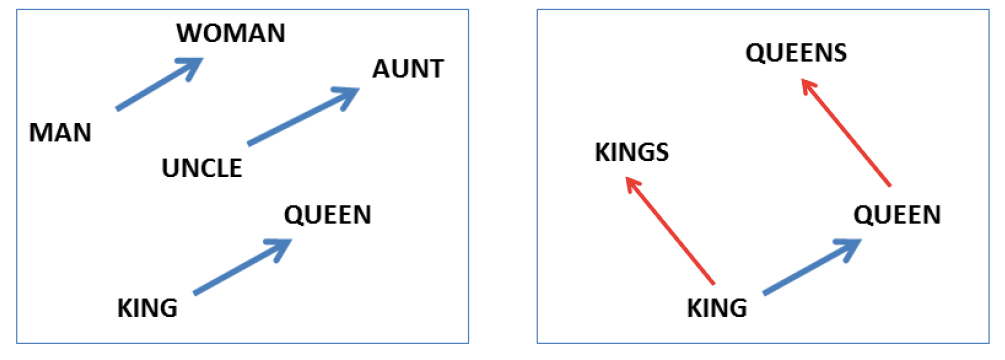
\includegraphics[width=14cm]{Images/word2vec.png}
	\centering
	\caption{Linguistic regularities preserved by the word2vec algorithm \cite{word2vec,mikolovDistirbutedRepresentationsOfWords}.}
	\label{fig:word2vec}	
\end{figure}

A similar algorithm for learning vectors is \emph{GloVe} (Global Vectors for Word Representation) \cite{glove}. GloVe is essentially a log-bilinear model with a weighted least-squares objective. The main intuition underlying the model is the simple observation that ratios of word-word co-occurrence probabilities have the potential for encoding some form of meaning.
The authors of \cite{linkingGloveWithWord2Vec} shows that GloVe and Skip-Gram model of word2vec, one explicitly factorizing a co-occurrence matrix and one implicitly factorizing a shifted-PMI matrix, are actually sharing similar objectives, though not completely the same.

It is important to note that the word-embedding techniques are using the fact that the order of words in text is important. This is not applicable for the non-target attributes within the datasets as the order is not important. We could easily permutate all the attributes and still argue that the information required to learn the features is still the same. In comparison, the order of words usually matters in the texts written by humans -- which is one of the reasons why the vector embeddings show such nice results.

The key factor in the performance of word2vec and similar methods is the size of the corpus. Common choice is up to one billion of words \cite{word2vec}.


There has also been ongoing research to use the vector embeddings on different domains than just natural languages. For example, \emph{protein-vectors} (ProtVec)~\cite{protvec} uses word2vec ideas.
The paper uses  Skip gram neural network to build a dense distributed representation for biological sequences. The method was evaluated by classifying protein sequences obtained from \emph{Swiss-Prot} \cite{uniprot} and outperformed existing classification methods. Furthermore, the method is applicable to other bioinformatics problem such as protein visualization, structure prediction, domain extraction, and interaction prediction.

\subsection{Kernels}
\label{section:kernels}
The kernel approach tackles the problem by looking at the similarities between objects. In general, kernel \cite{kernels} is a function taking two objects and returning a measurement:

\begin{definition}
	Let $\Omega$ be a set. Then \emph{kernel} K is a real-valued function of two variables from $\Omega$, i.e., 
	\begin{equation}
	\Omega \times \Omega \rightarrow \mathbb{R}
	\end{equation}
\end{definition}

To get a similarity, only the so called dot-product kernels are usually considered:
\begin{definition}
	Let $\Omega$ be a set. Then \emph{dot-product kernel} K is a real-valued function of two variables from $\Omega$ satisfying
	\begin{equation}
	K(x,y) = \langle\phi(x), \phi(y)\rangle_{\mathbb{V}},
	\end{equation}
	where $\phi$ is a \emph{feature map} $X \rightarrow \mathbb{V}$ and $\langle\cdot,\cdot\rangle_{\mathbb{V}}$ is an inner product on $\mathbb{V}$.
\end{definition}

If $\Omega$ is a space of real vectors, the dot product is a commonly considered inner product, and we can easily get so called linear kernel just by using the dot product:
\begin{equation}
K(x,y) = x^ty, \forall x,y \in \mathbb{R}^n.
\end{equation}
It is possible to use $\phi$ for rescaling and increase of dimensions. For instance, the polynomial kernel defined as 
\begin{equation}
K(x,y) = (x^ty+b)^n, x,y \in \mathbb{R}^n, r > 0, n \in \mathbb{N}, n > 0.
\end{equation}
computes the product in $\binom {d+2}2$-dimensional feature space where $d$ is a dimension of input vectors and $b$ is a parameter describing the influence of higher order terms versus lower order terms. For example, for $n=2$ the product is given by the (implicitly defined) mapping 
\begin{align*}
&\phi(\langle x_1,\dots,x_n\rangle)= \\
&\langle x_1^2,\dots, x_1^n,\sqrt{2}x_1x_2,\sqrt{2}x_1,x_3,\dots, \sqrt{2}x_{n-1}x_n,\sqrt{2b}x_1,\dots,\sqrt{2b}x_n,c\rangle.
\end{align*}

Other popular kernel is the so called \emph{radial basis function} (RBF) kernel:
\begin{equation*}
	K(x,y)=e^{-\gamma||x-y||^2},
\end{equation*}
where $\gamma$ is a parameter of the kernel.

What makes the kernel approach particularly interesting is that $\Omega$ can be an arbitrary set, not just real numbers. If we can define a mapping $\Omega$ to some space with inner product, we can  have a kernel even for objects with variable structure.

For instance, strings over some alphabet have variable structure as they can be of arbitrary length.
One of the kernels defined over strings is string subsequence kernel \cite{stringSubsequenceKernel}, which defined the similarity of two strings by the number of their common subsequences (not-necessarily contiguous):

\begin{definition}
	Let $\mathbb{A}$ be an alphabet and $x,y \in \mathbb{A}$. The \emph{string subsequence} kernel is defined as:
	\begin{equation*}
	K(x,y)=\sum_{u \in \mathbb{A}^n}\sum_{i: u = x[i]}\sum_{j: u = y[i]} \lambda ^{l(i)+l(j)},
	\end{equation*}
	where $\mathbb{A}^n$ is the set of all strings of length $n$, $s[i]$ is a subsequence of $s$ given by some set of indices $i$, $\lambda$ is a decay factor and $l(i)$ denote the total length of $s[i]$ in $s$ -- the biggest index in $i$ minus the smallest index in $i$ plus one.
\end{definition}
While this computation appears very expensive, recursive computation can be reduced to $\mathcal{O}(n|x||y|)$ \cite{stringSubsequenceKernel}. 

Another example of the string kernel is a spectrum kernel \cite{spectrumKernel}, which bases the similarity on common substrings of some predefined length.
\begin{definition}
	Given a number $k \ge 1$, the \emph{k-spectrum} of an input sequence is the set of all the k-length (contiguous) subsequences that it contains.
\end{definition}
We defined a kernel with a feature map indexed by all possible subsequences $a$ of length $k$ from alphabet $\mathbb{A}$.
\begin{definition}
	\emph{$K$}-spectrum kernel is defined as:
	\begin{equation*}
	K(x,y) = \langle (\phi_a(x))_{a \in \mathbb{A}^k}, \phi_a(y))_{a \in \mathbb{A}^k} \rangle,
	\end{equation*}
	where $\phi_a(x)$ denotes number of times $a$ occurs in $x$.
\end{definition}
A very efficient method for computing spectral kernel is to build a suffix tree for the collection of $k$-length subsequences of $x$ and $y$, obtained by moving a $k$-length sliding window across each of $x$ and $y$. At each depth-$k$ leaf node of the suffix tree, store two counts, one representing the number of times a $k$-length subsequence of $x$ ends at the leaf, the other representing a similar count for $y$. Note that this suffix tree has $\mathcal{O}(kn)$ nodes. Using a linear time construction algorithm for the suffix tree \cite{onlineConstructionOfSuffixTrees}, we can build and annotate the suffix tree in  $\mathcal{O}(kn)$ time. Now we calculate the kernel value by traversing the suffix tree and computing the sum of the products of the counts stored at the depth-$k$ nodes. The overall cost is thus $\mathcal{O}(kn)$. 

We would like to mention another string kernel called local alignment as it directly influenced our work.
\begin{definition}
	An \emph{alignment} (with gaps) $\pi$ of $p \ge 0$ positions between two sequences $x,y$ is a pair of $p$-tuples:
	\begin{equation*}
	\pi = ((\pi_1(1),\dots,\pi_1(p),\pi_2(1),\dots,\pi_2(p)) \in \mathbb{N}^{2p}
	\end{equation*}	
	that satisfies
		\begin{equation*}
		1 \le \pi_1(1) < \pi_1(2) < \dots \pi_1(n) \le |x|
		\end{equation*}
		\begin{equation*}
		1 \le \pi_2(1) < \pi_2(2) < \dots \pi_2(n) \le |y|
		\end{equation*}
\end{definition}
We can score the alignments as follows:
\begin{definition}
The \emph{local alignment} score of an alignment $\pi$ is equal to
\begin{equation*}
s_{S,g}(\pi) = \sum_{i=1}^{|\pi|}S(x_{\pi_1(i)},y_{\pi_2(i)}) - \sum_{i=1}^{|\pi|-1}
[g(\pi_1(i+1)-\pi_1(i))+g(\pi_2(i+1)-\pi_2(i))],
\end{equation*}
where S is a substitution matrix encoding score for aligning letters with other letters and $g$ is a gap penalty function.
\end{definition}
The \emph{Smith-Waterman} (SW) score is a local alignment score of the best alignment:
\begin{equation*}
SW_{S,g} = \max_{\pi \in \Pi(x,y)}s_{S,g}(\pi).
\end{equation*}
The SW score can be calculated in $\mathcal{O}(|x||y|)$ by dynamic programming with Smith-Waterman algorithm \cite{smithWaterman}.
\begin{equation}
SW(i,j)= \max
	\begin{cases}
	0, \\
	SW(i-1,j)+S(x_i, y_j), \\
	\max_k{SW(i-k,j)-g(k)}, \\
	\max_l{SW(i,j-l)-g(l)}. \\
	\end{cases}
\end{equation}
$SW(i,j)$ stands for the similarity of two segments ending in $x_i$ and $y_j$ respectively.

Unfortunately, SW score does not have to be a valid inner-product kernel~\cite{smithWatermanKernel}. However, a convolution kernel can be defined as follows:
\begin{equation}
K_{LA}^{(\beta)}(x,y) = \sum_{\pi \in \Pi(x,y)}e^{\beta s_{S,g(\pi)}},
\end{equation}
where $\beta$ is a parameter. It can be shown that the SW score is approached by the limit:
\begin{equation}
\lim_{\beta \rightarrow \infty} \frac{1}{\beta}\ln(K_{LA}^{(\beta)}(x,y)) = SW(x,y).
\end{equation}
 Furthermore, it can be shown that if there is no gap penalty a SW score is a kernel \cite{swNoGapKernel}.

Another domains where kernels were applied is the space of graphs \cite{graphKernels} and images \cite{imageKernels}. Again, we cannot apply string or graph kernels directly to the dataset space as the order of character or vertices matters. 

Having an inner product kernel has many advantages. Computation of the inner product kernel can be carried out without explicitly using the $\phi$ function and computing the inner product. Mapping to the feature space can be very expensive or not feasible at all. For example, the RBF kernel with $\gamma = 1$ is actually computing the inner product in an infinite dimensional feature space:
\begin{equation*}
e^{-||x-y||^2} = \sum_{j=0}^{\infty}\frac{(x^Ty)^j}{j!}e^{(-\frac{1}{2}||x||^2)}e^{(-\frac{1}{2}||y||^2)}.
\end{equation*}
Such computation of inner product in the feature space using only values in the input space is sometimes being referred to as a \emph{kernel trick}.

Many methods benefit from the kernel trick or can be extended to do so. For example, \emph{support vector machine} (SVM) \cite{svm} can use the kernel to separate non-linearly separable sets by performing the separability in the feature space instead. The ability of kernels to be used in such a way is demonstrated in Figure \ref{fig:nonlinearitythroughkernels} by using the scikit-learn library \cite{scikit-learn}. First, two categories of points are generated -- blue points distributed over the circle with some small noise and red circles distributed around the circle with bigger radius. Clearly, the blue set is not linearly separable from the red set. Using another method enhanceable by the kernel trick -- \emph{kernelized PCA} with the RBF kernel \cite{kernelizedSVM} -- we can achieve the linear separability.

\begin{figure}
	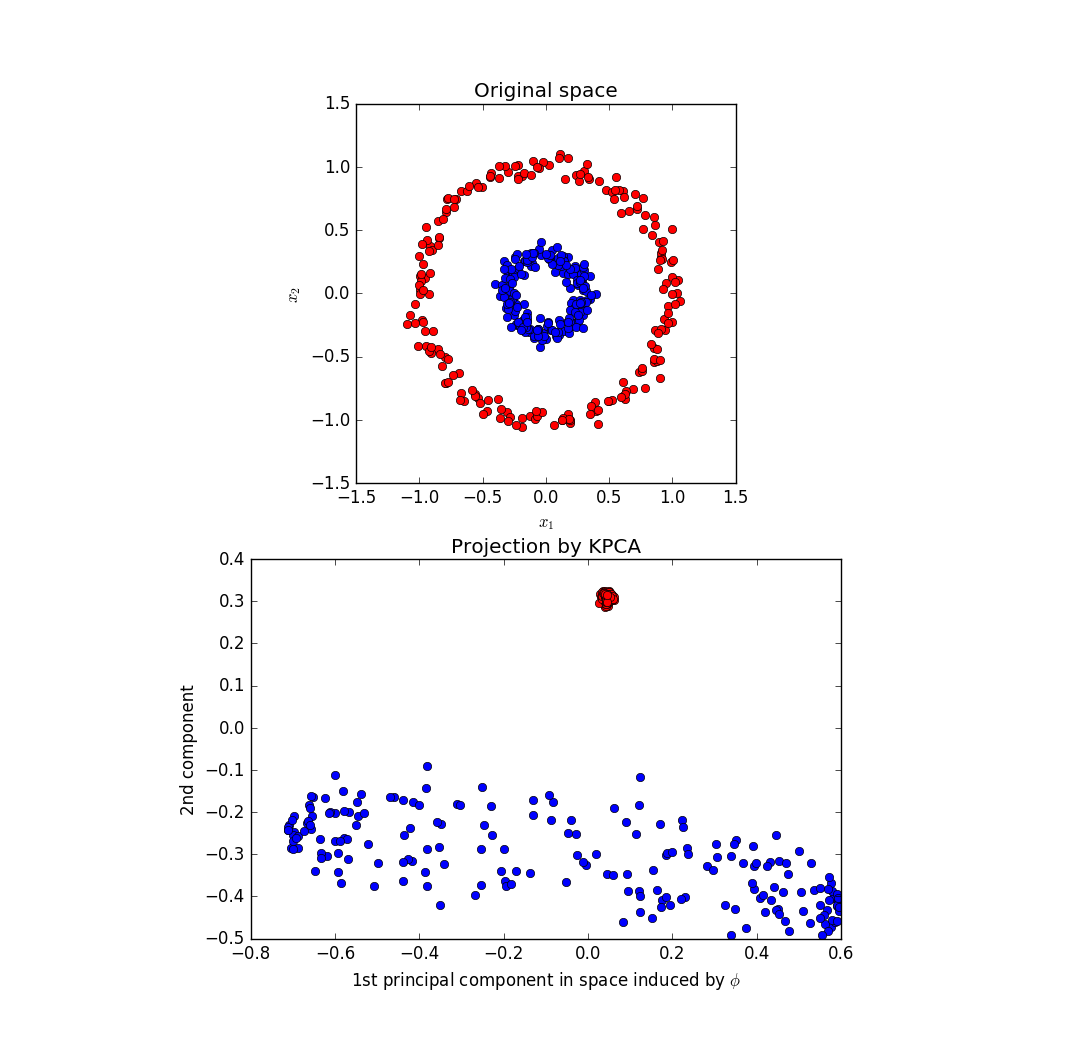
\includegraphics[width=16cm]{Images/nonlinearitythroughkernels.png}
	\centering
	\caption{Example of using the kernelized PCA in the scikit-learn library \cite{scikit-learn} to make the data linearly separable.}
	\label{fig:nonlinearitythroughkernels}	
\end{figure}
The kernelized PCA opens many options as it can map arbitrary space with kernel to the vector of the desired length. Reducing the dimensions to two or three is especially useful as it can be visualized easily.

Metalearning is also used to aid the methods with kernels as choosing a right kernel can be crucial to solve the problem at hand. Authors of \cite{kernelSelectionMetalearning} use meta-learning to select the right kernel for SVM by measuring the problem characteristics using classical, distance and distribution-based statistical information. In \cite{kernelLearningByTransferLearning} the kernel is automatically selected based on knowledge transferred from the results on related data.

\section{Non-propositional Approach to Metalearning}
\label{section:NonpropositionalApproachToMetalearning}

All of the methods for algorithm selection problem discussed so far used the propositional approach -- every dataset was represented by the metadata vector of fixed size. However, the problem is highly non-propositional as the number of attributes varies throughout the datasets. According to the authors of \cite{BrazdilMetalearning-2009}, the most common approach to deal with this problem is to do some form of aggregation, for example use mean skewness as an aggregation of every attribute with skewness. It is expected that important information will be lost in the process. In \cite{jaOndraMetadataMetric}, we partially addressed the problem by adding the special attribute metadata. First, we identified the most significant attributes. The significance of attribute was identified by the \emph{joint entropy} of a target class and attribute:
\begin{equation}
H(A,C) = - \sum_{v \in Val(A)}\frac{n(A(v))}{n}
\sum_{t \in Val(C)}\frac{n_t(A(v))}{n(A(v))}\log_2\frac{n_t(A(v))}{n(A(v))},
\end{equation}
where $n$ is the number of observations, $n(A(v))$ is the number of observation with the value $v$ of the attribute and $n_t(A(v))$ is the number of observations with the value $v$ of the attribute and with the value $t$ of the target attribute.
For the continuous attributes (for them the direct entropy computation is not desirable) the discretization of the values was used instead. We then chose a number $k$ and the attribute metadata of $k$ most significant attributes were added to the propositional representation of the datasets. We specifically used entropy (see Equation \ref{equation:entropy}) of the $i$-th most significant attribute.
It is however easy to extend the approach with the arbitrary attribute metadata.

Alternatively, in \cite{KalousisDesignImplementationAndPerfromance} two measures of association are used, one for continuous attributes and one for discrete ones. For continuous attributes, the absolute value of the correlation coefficient is used, for discrete attributes, the \textit{Goodman and Kruskal's tau} \cite{AgrestiCategoricalDataAnalysis} coefficient also known as the concentration coefficient is used. The problem of the various number of attributes is dealt with by introducing a histogram of these attributes with the fixed number of bins.

Both the approaches above are merely pushing the problem further. As we have chosen fixed number of most significant attributes or bins, what happens if we have to deal with datasets with billion times more attributes than the number of bins?

Kalousis et al. \cite{RepresentationalIssuesInMetalearning} solve the problem of varying attributes by defining a distance measure on the attribute space. The dataset distance is then similar to the distances used in clustering -- either \emph{Single Linkage Based Similarity} (similarity taken is the maximum similarity between the attributes) or \emph{Average Linkage Based Similarity} is used. Attribute similarity is calculated as 1 minus the Manhattan distance defined on the attribute metadata. This can handle the non-propositional approach and the authors demonstrated that such distance function is useful in metalearning. However, we can still imagine datasets that are very different but whose Single Linkage Based Similarity is high (one common attribute, many very different attributes) and similar datasets whose Average Linkage Based Similarity is low (many similar attributes but distant from others).
A possible explanation is that the Single Linkage Based Distance  does not necessarily produce a metric:
\begin{observation}
	Given arbitrary metric $\attributeDistance$ on the attribute space whose cardinality is at least two there exist datasets $a,b,c$ such that the distance between datasets $\globalDistance$ induced by Single Linkage Clustering 
	$$\globalDistance(a,b)=\min_{i, e_i \in a, j, e_j \in b}(\attributeDistance(e_i,e_j))$$ is not a metric on the dataset space.
	\begin{proof}
	The attribute space has at least two distinct elements, we will call them $e_1, e_2$. Let $a=\{e_1\}$, $b=\{e_2\}$ and $c=\{e_1, e_2\}$. Then $$\globalDistance(a,c)+\globalDistance(b,c) = 0+0 < \globalDistance(a,b),$$
	which breaks the triangle inequality.
	\end{proof}	
\end{observation}

We can also find the similar counterexample for the Average Linkage Based Distance:
\begin{observation}
	Given arbitrary metric $\attributeDistance$ on the attribute space whose cardinality is at least two there exist datasets $a,b$ such that the distance between datasets $\globalDistance$ induced by the Average Linkage Clustering $$\globalDistance(a,b)=\frac{1}{|a||b|}\sum_{i, e_i \in a}\sum_{j, e_j \in b}\attributeDistance(e_i,e_j))$$ is not a metric on the dataset space.
	\begin{proof}
		The attribute space has at least two distinct elements, we will call them $e_1, e_2$. Let $a=b=\{e_1, e_2\}$. Then $$\attributeDistance(a,b)=\frac{1}{4}(0+\attributeDistance(e_1, e_2)+0+\attributeDistance(e_,e_1))=\frac{1}{2}\attributeDistance(e_1,e_2)>0,$$
		which breaks the coincidence axiom.
	\end{proof}	
\end{observation}

\section{Distance Using Attributes}
\label{section:distanceUsingAttributes}
As discussed in the beginning of this chapter, ability to process unstructured data can significantly improve the tasks defined on those data as we can use bigger palette of approaches. Unfortunately, the methods proposed on the strings and graph spaces are not out of the box applicable to the space of datasets but rather can serve as an inspiration. For example, the Smith-Waterman algorithm looks interesting, but it was designed with the fact that the order of letter matters in mind. With the datasets, it should not matter if we permutate the attribute. The target function should be learnable all the same as we can preprocess the attributes by inverse permutation. The non-propositional approaches reviewed in the previous section are either losing information or lacking properties usually important for the distance functions.

Authors of \cite{DistancesAndIndefiniteKernelsForTheSetsOfObjects} review possible ways of using the distance measures defined on $\mathbb{X}$ in
order to define distance measures on the power set $2^\mathbb{X}$ of $\mathbb{X}.$
The most promising is the distance measure defined as follows:
\begin{equation}
D_M(A,B) = \min_{R_i \in R}{(\sum_{(a_k, b_j) \in R_i}{\attributeDistance(a_k, b_j)}+(|B \setminus R_i(A)|+|A \setminus R_i^{-1}(B)|)\frac{M}{2})},
\end{equation}
where $\attributeDistance$ is a distance between elements of some space $\mathbb{S}$, $A,B \subseteq \mathbb{S}$, $R_i$ is a matching (each element at most once) on $A \times B$, and $M$ is a maximum distance of $\attributeDistance$ on $\mathbb{S}$. $D_M$ can be also viewed as a distance that finds optimal mapping between elements of $A,B$ and can decide to omit some elements by getting $\frac{M}{2}$ penalty.
Authors of  \cite{polynomialTimeComputableMetricBetweenPointSets} prove that the $D_M$ is a metric if $\attributeDistance$ is a metric. Furthermore, $D_M$ is computable in the polynomial time.
We can treat datasets as composed by attributes and use $D_M$ by defining a distance $\attributeDistance$ on attribute space. However, there are still reasons that render this approach impractical for metalearning.
The distance measure $D_M$ requires $M$. The computation of $M$ may not be feasible or not known in advance, especially if the attribute distance was not normalized. Additionally, some attributes may be more significant than the others. Not matching some insignificant attributes because of fewer attributes in the second dataset (for example with low entropy for predicting the target attribute) will still result in $\frac{M}{2}$ distance. Also, algorithm can decide not to match some attributes with high difference and get only $\frac{M}{2}$ penalty. For example, when comparing two datasets with single attributes, the results will be the same if the attributes are really distant ($M$) or somewhat distant ($\frac{M}{2}$). In both cases the $D_M$ will return $\frac{M}{2}$.

In this section, we propose several approaches that can handle the non-propositional dataset representations without any trade-offs. We have already published their descriptions and experiments validating their asset in ~\cite{diplomka,jaIcannga2013,SSCI2014,jaCEC2015,jaSSCI2015}. Each one is based on the idea of attribute aligning where the order of attributes is not important. By supplying a function measuring the distance between individual attributes (like in \cite{RepresentationalIssuesInMetalearning}), we could try to align the attributes in the way that minimizes the sum of distances between aligned attributes. To avoid confusion, we will always denote attribute distance measure as $\attributeDistance$. The name was not chosen randomly. The upper case $\globalDistance$ -- as always -- will denote the final dataset distance measure. As we will see, we will piece $\globalDistance$ out of smaller $\attributeDistance$s, hence the name.

Although we are aiming to handle the non-propositional approach, we will start with propositional situation to describe the approach, and extend it later to handle varying amount of attributes.
For now let us suppose that there is the same number of attributes in every dataset (and hence the same number of attribute metafeatures).

\begin{definition}
Given a distance function between attributes $\attributeDistance$, two datasets $a,b$ and a bijection $f$ between the attributes of $a,b$ we define the dataset distance induced by the bijection between the datasets as:
\begin{equation}
\globalDistance_f(a,b)=\sum_{k=1}^{n}{(\attributeDistance(a_k,f(a_k)))},
\label{eq:attdist}
\end{equation}
where $a_k$ is the $k$-th attribute of $a$ and $f(a_k)$ corresponding attribute in dataset b given by the bijection $f$.
We will sometimes refer to the $\globalDistance_f$ as the \emph{cost} of $f$.
\end{definition}
We would like to match the attributes as best as possible to get the lowest possible distance $\globalDistance_f$, so optimally we are looking for $f^*$:
\begin{equation}
f^*= \mathrm{argmin}_f(\globalDistance_f).
\label{eq:argmin}
\end{equation}
We will denote $f^*$ as an optimal alignment.

From this, the general distance between datasets can be derived:
\begin{equation}
\globalDistance(a,b) = \globalDistance_{f^*}(a,b).
\end{equation}

Now suppose that the number of attributes is different. We transform this case to the previous one by adding dummy attributes into the dataset with less attributes. We can think of a dummy attribute in a similar way as of a gap penalty in the Smith-Waterman algorithm. There are two approaches how to do this. Suppose $\mathbb{A}$ is a space of attributes. Either $dummy \in \mathbb{A}$ or $dummy \notin \mathbb{A}$. In the former case, nothing is needed, as the distance function between attributes is already defined if the $\dummy$ attribute is on the input. In the latter case, it is needed to extend the distance function by defining the distance between a regular attribute and the $\dummy$ one.
In the further text, we will refer to the attribute space with the $\dummy$ attribute as to the \emph{extended attribute space}. If it is clear from the context, we will sometimes refer to extended attribute space simply as attribute space. $Dummy$ attribute will be referred to as $\dummy$ or specifically to $\dummyinside$ if the dummy attribute is already in the attribute space and $\dummyoutside$ if the attribute is newly created.
We will discuss the pros and cons of these approaches as well as how to choose the right attribute for the $\dummy$ one, and how to define the distance between a regular attribute and a $\dummy$ one respectively in Section \ref{section:theoreticalProperties}.

From now on, we can suppose that if we are aligning two datasets that they have the same number of attributes, and that one dataset was to some extent enriched with some number of $\dummy$ attributes, so the amount of attributes matches.

There are $n!$ bijections from $a$ to $b$. It is costly to enumerate them, so it is desired to eliminate some of the bijections in advance. In this work, we came up with two approaches that vary in the generality of the attribute distance and computational complexity.
\begin{definition}
\emph{Evaluation function} $\sigma$ is a function mapping attributes to $\mathbb{R}$.
\end{definition}

In our first approach, we suppose we have $\sigma$ (for example, number of distinct values), and the attribute distance is defined as follows:
\begin{equation}
\attributeDistance(a_k, f(a_k))=|\sigma(a_k)-\sigma(f(a_k))|.
\label{eq:sigma}
\end{equation}

\begin{theorem}
Given datasets $a,b$ and a bijection $f$, if we sort $a$ and $b$ by $\sigma$ in the ascending order obtaining $a',b'$ we can find $f'$ such that
\begin{equation}
\globalDistance_{f'}(a',b')=\globalDistance_f(a,b).
\label{eq:df}
\end{equation}
\end{theorem}
\begin{proof}
Let $\pi _{a}$, $\pi _{b}$ be the permutations used to sort $a,b$. Define $f'$ as follows:
\begin{equation}
f'(a'_i)=\pi _{b}(f(\pi _{a}^{-1}(a'_i))).
\label{eq:fai}
\end{equation}
We have to prove that for every $k$ there is $j$ such that $|\sigma(a_k)-\sigma(f(a_k))|=|\sigma(a'_j)-\sigma(f'(a'_j))|$. As a candidate for $j$ we take such $j$ that $a'_j=\pi_{a}(a_k).$ Such $j$ exists and it is unique as $\pi_{a}$ is a permutation. Observe that sorting permutation does not affect $\sigma.$ Therefore $\sigma(a'_j)=\sigma(\pi_{a}(a_k))=\sigma(a_k).$ %Mark index of $f(a_k)$ as $z$. 
Directly from the observation the following equation can be derived: 
\begin{equation}
\sigma(f'(a'_j))=\sigma(\pi _{b}(f(\pi _{a}^{-1}(a'_j))))= \sigma(f(\pi _{a}^{-1}(a'_j)))=\sigma(f(a_k)),
\label{eq:faj}
\end{equation}
which concludes the proof as the $j$ is unique and it always exists.
\end{proof}

\begin{corollary}
We can exclusively use this canonical representation and without the loss of generality, suppose that $a,b$ are sorted by $\sigma$.
\end{corollary}

\begin{definition}
We say that the bijection $f$ is the \emph{identity alignment} if $\forall i,a_i \in a:f(a_i)=b_i$. 
\end{definition}
The example of the identity alignment is shown in Figure~\ref{fig:identity}.
\begin{figure}
	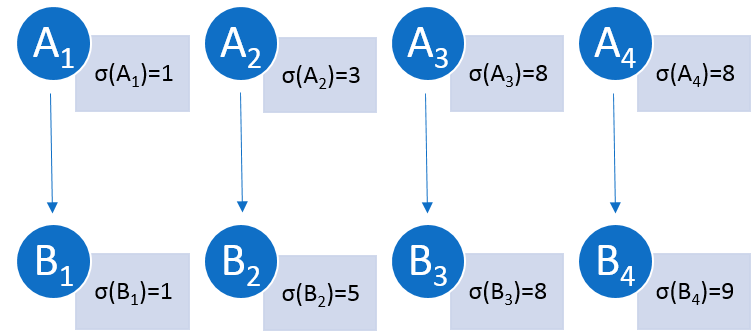
\includegraphics[width=9.5cm]{Images/identity.png}
		\centering
	\caption{Example of the identity alignment. If the attributes are sorted by $\sigma$, each attribute is aligned to the attribute with the same order.}
	\label{fig:identity}	
\end{figure}

\begin{theorem}
\label{mainproof}
Identity alignment is optimal.
\end{theorem}
\begin{proof}
Given the bijection $f$ that is not an identity alignment and is optimal, we will show that it can be either transformed to identity alignment or it is not optimal, which leads to a contradiction. Find the lowest $i$ such that $f(a_i)\neq b_i $. Such $i$ exists, because $f$ is not an identity alignment. We mark the index of attribute $f(a_i)$ as $z$. Because $f$ is a bijection, we can find $j$ such that $f^{-1}(b_i)=a_j$. Take a bijection $f'$ that is the same as $f$ with the exception of arguments $i$ and $z$:
 \begin{eqnarray}
    f'(a_i)&=b_i, \nonumber \\
    f'(a_j)&=b_z.
    \end{eqnarray}
In other words, $f'$ is more similar to identity alignment than $f$. The whole transformation is shown in Figure~\ref{fig:transformation}. 
\begin{figure}	
		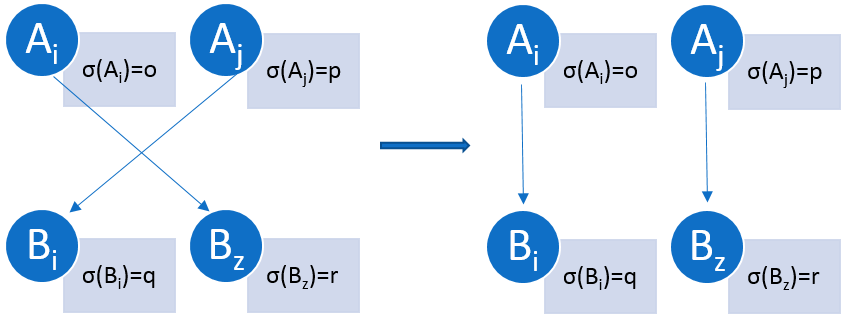
\includegraphics[width=9.5cm]{Images/transformation.png}
		\centering
	\caption{Example of transformation. Find attributes that falsify identity alignment and switch them. At least one less pair of attributes now falsifies the identity alignment.}	
	\label{fig:transformation}	
\end{figure} 

We have to verify that:
 \begin{align}
    d_f &\geq d_{f'}. \\
    \sum_{k=1}^{n}{(|\sigma(a_k)-\sigma(f(a_k))|)}     &\geq \sum_{k=1}^{n}{(|\sigma(a_k)-\sigma(f'(a_k))|)}.
    \end{align}
    
The $d_f$ and $d_f'$ differs only in positions $i$ and $j$. Thus we can simplify the equation to:
\begin{align}
    \sum_{k \in {i,j}}{(|\sigma(a_k)-\sigma(f(a_k))|)} 
    &\geq \sum_{k \in {i,j}}{(|\sigma(a_k)-\sigma(f'(a_k))|)}.  
\end{align}    
\begin{align}    
    &|\sigma(a_i)-\sigma(b_z)|+|\sigma(a_j)-\sigma(b_i)| \geq |\sigma(a_i)-\sigma(b_i)|+|\sigma(a_j)-\sigma(b_z)|. 
\end{align} 
If we denote values $\sigma(a_i),\sigma(a_j),\sigma(b_i),\sigma(b_z)$ as $o,p,q,r$, we can simplify the equation further:
\begin{equation}
|o-r|+|p-q|\geq |o-q|+|p-r|.
\label{eq:targetCondition}
\end{equation}
Because we use sorted canonical representation and because of the fact we have taken the lowest $i$ possible we know that:
\begin{equation}
o\leq p,
\label{eq:op}
\end{equation}
\begin{equation}
q \leq r.
\label{eq:qr}
\end{equation}
There are 6 possible orderings of $o,p,q,r$ that fulfils these two equations. The enumeration of these 6 cases is in Table \ref{table:caseEnum}.

\begin{table}[htbp]
\caption{Equation \ref{eq:targetCondition} holds for every possible case.}
\label{table:caseEnum}
\centering
\begin{tabular}{ |c | c | c |c | }
  \hline
  ORDER & $|r-o|+|q-p|$ & $|q-o|+|r-p|$ & $\geq$ \\
  \hline                       
  opqr & $|q-r|+2*|q-p|+|p-o|$ & $|q-r|+2*|q-p|+|p-o|$ & $=$ \\
  oqpr & $|r-p|+2*|q-p|+|q-o|$ & $|q-o|+|r-p|$ & $\geq$\\
 oqrp & $2*|q-r|+|q-o|+|r-p|$ & $|q-o|+|r-p|$ & $\geq$\\
  qopr & $|r-p|+|q-o|+2*|p-o|$ & $|q-o|+|r-p|$ & $\geq$\\
  qorp & $2*|r-o|+|q-o|+|r-p|$ & $|q-o|+|r-p|$ & $\geq$\\
  qrop & $2*|r-o|+|q-r|+|p-o|$ & $2*|r-o|+|q-r|+|p-o|$ & $=$\\
  \hline  
\end{tabular}
\end{table}
In every presented case, the $f'$ is at least as good as $f$, and the position $i$ no longer falsifies the identity alignment. If $f'$ is still not the identity alignment, we can repeat the previous step until we get an identity alignment because the number of attributes is finite.
\end{proof}

\begin{corollary}
Based on Theorem \ref{mainproof}, a more efficient algorithm for the attribute alignment can be derived with the complexity of alignment equal to $\mathcal{O}(n\log(n))$, where $n$ is the number of attributes.
\end{corollary}

%http://get-software.net/macros/latex/contrib/algorithm2e/doc/algorithm2e.pdf
\IncMargin{1em}
\begin{algorithm}
\SetKwInOut{Input}{input}\SetKwInOut{Output}{output}
\tcp{Pseudocode for an attribute alignment algorithm with constrained attribute distance function running in $\mathcal{O}(n\log(n))$.}
\Input{a $\leftarrow$ List of attributes}
\Input{b $\leftarrow$ List of attributes}
\Input{$\sigma \leftarrow$ Attribute evaluation function: $\mathbb{A}\rightarrow \mathbb{R}$}
\Output{Distance between a and b}
\BlankLine
Add dummy attributes into the list with less attributes\;
Sort both list of attributes by $\sigma$\;
totalDistance $\leftarrow 0$\;
\For{$i\leftarrow 0$ \KwTo $i < \text{len}(a)$}{
totalDistance $\leftarrow$ $|\sigma(a[i])-\sigma(b[i])|$\;
}
\Return totalDistance\;
\caption{Attribute alignment}
\label{algo:attributeAlignmentMasterThesis}
\end{algorithm}\DecMargin{1em}

The pseudocode is outlined in Algorithm \ref{algo:attributeAlignmentMasterThesis}.

From the algorithm, the total computational complexity can be inferred. The sorting can be done in $\mathcal{O}(n\log(n))$, where $n$ is the number of attributes. The enumeration can be done in $\mathcal{O}(n)$, the evaluation of $\sigma$ for every attribute takes $\mathcal{O}(nc(\sigma))$~steps, where $c(\sigma)$ is a cost of calling the evaluation function for a single attribute. Therefore, the total complexity of Algorithm \ref{algo:attributeAlignmentMasterThesis} is  $\mathcal{O}(n(\log(n)+c(\sigma))).$

In our second approach, we allow arbitrary function $\attributeDistance$ measuring the distance between two attributes. Given two datasets $a,b$ and attribute distance function $\attributeDistance$, a distance matrix $M$ can be easily built up:
\begin{equation}
M_{i,j} = \attributeDistance(a_i,b_j).	
\end{equation}
We can see the distance matrix $M$ as the cost function and the aligning of attributes as an assignment, which leads to an assignment problem. The assignment problem is well known. The polynomial algorithm -- in the graph theory known as the Hungarian algorithm -- solving the assignment problem in $\mathcal{O}(n^4)$ was described in \cite{KuhnHungarian}. The $\mathcal{O}(n^3)$ implementation of the Hungarian algorithm was later published in \cite{KarpHungarian}.
Before the algorithm itself we will state few definitions needed. Given a graph $G = (V, E)$:  

\begin{definition}
A \emph{matching} is a subset $M \subseteq E$ such that $\forall v \in V$ at most one edge in $M$ is incident upon V.
\end{definition}

\begin{definition}
A \emph{perfect matching} is an $M$ in which every vertex is adjacent to some edge in $M$.
\end{definition}

\begin{definition}
A vertex \emph{labelling} is a function $l:V\mapsto R.$
\end{definition}

\begin{definition}
Vertex $v$ is \emph{matched} if it is an endpoint of edge in $M$, otherwise it is \emph{free}.
\end{definition}

\begin{definition}
The \emph{equality graph} with the respect to the labelling l is $G=(V,E_l)$, where $E_l=\{(x,y)|x,y \in V, l(x)+l(y)=w(x,y)\}.$
\end{definition}

\begin{definition}
A path is \emph{alternating} if its edges alternate between $M$ and $E \setminus M$.
\end{definition}

\begin{definition}
An alternating path is \emph{augmenting} if both endpoints are free.
\end{definition}

\begin{definition}
Define \emph{neighbour} of $u \in V$ and set $S\subseteq V$ to be:
\begin{equation}
N_l(u)={v:(u,v)\in E_l}, N_l(S)=\cup_{u\in S}N_l(u).
\label{eq:nlu}
\end{equation}
\end{definition}
%\pagebreak
Given the definitions above, the pseudocode for the Hungarian algorithm can be outlined, as per Algorithm \ref{algo:hungarianAlgorithm}.

\IncMargin{1em}
\begin{algorithm}
\SetKwInOut{Input}{input}
\SetKwInOut{Output}{output}
\tcp{Pseudocode of the Hungarian Algorithm solving assignment problem in $\mathcal{O}(n^3)$.}
\Input{$(X \cup Y,E)$ $\leftarrow$ Weighted bipartite graph }
\Output{Minimal assignment}
\BlankLine
Generate initial labelling $l$ and matching $M$ in $E_l.$ \;
\While{\upshape $M$ is not perfect}{
	$u \leftarrow$  pick free vertex $\in X$\;
	$S \leftarrow$  $\left\{u\right\}$\;
	$T \leftarrow$  $\left\{\right\}$\;
	\If{$N_l(S)=T$}{
	update labels (forcing $N_l(S)\neq T$) \;
	$a_l \leftarrow \min_{s \in S,y\notin T}(l(x)+l(y)-w(x,y)) $\;
	$
	 l'(v) \leftarrow
	 \begin{cases}
	 l(v)-a_l; \mbox{ if } v \in S, \\
	 l(v)+a_l; \mbox{ if } v \in T, \\
	 l(v); \mbox{ otherwise}.
	 \end{cases}
	$
	}
	\If{$N_l(S)\neq T$}{
	pick $y \in N_l(S)-T$\;
	If $y$ free, $u-y$ is augmenting path. Augment $M$ and go to 2\;
	If $y$ matched, say to $z$, extend alternating tree: \\ $S \leftarrow S\cup {z},T \leftarrow T\cup {y}$. Go to 6\;
	}
}

\Return minimalAssignment\;
\caption{Hungarian algorithm}\label{algo:hungarianAlgorithm}
\end{algorithm}\DecMargin{1em}


We can use this algorithm to find the best assignment of the attributes. From the assignment the total distance between attributes can be computed as the sum of individual distances defined by the alignment as already seen in Algorithm \ref{algo:attributeAlignmentMasterThesis}. If  $\attributeDistance$ was defined in the same manner as in the first approach, we would get the same result (Algorithm \ref{algo:attributeAlignmentMasterThesis} is a special case of Algorithm \ref{algo:attributeAlignmentHungarian}). The difference is that this version allows for an arbitrary function measuring distance between attributes as an input.

For the sake of generalization, we will define $IAttributeDistance$ interface that will represent such attribute distance. This interface is outlined in Algorithm \ref{interface:IAttributeDistance}. The total complexity of the algorithm depends on the complexity of this function and is $\mathcal{O}(n^3+n^2\sigma(n))$, where $n$ is the number of attributes and $\sigma(n)$ is the complexity of the attribute distance function. The whole algorithm that uses the Hungarian Algorithm and $IAttributeDitance$ is outlined in Algorithm \ref{algo:attributeAlignmentHungarian}.

\IncMargin{1em}
\begin{algorithm}
	\SetKwInOut{Input}{input}
	\SetKwInOut{Output}{output}
	\tcp{Interface for measuring distance between two attributes.}
	\Input{$a \leftarrow$ First attribute}
	\Input{$b \leftarrow$ Second attribute}
	\Output{ $d \in \mathbb{R}, d$ is an attribute distance $\attributeDistance$ between $a, b$. }
	\BlankLine
	\caption{$IAttributeDistance$: Dataset distance interface}
	\label{interface:IAttributeDistance}
\end{algorithm}\DecMargin{1em}

\IncMargin{1em}
\begin{algorithm}
\SetKwInOut{Input}{input}\SetKwInOut{Output}{output}
\tcp{Pseudocode for an attribute alignment algorithm using Hungarian Algorithm for the alignment.}
\Input{$a \leftarrow$ First list of attributes}
\Input{$b \leftarrow$ Second list of attributes}
\Input{$\attributeDistance$ $\leftarrow$ $IAttributeDistance$ Function}
\Output{Distance between $a$ and $b$}
\BlankLine
Add dummy attributes into the list with less attributes\;
$M[i,j] \leftarrow \attributeDistance(a[i], b[j])$\;
assignments $\leftarrow$ HungarianAlgorithm($M$)\;
totalDistance $\leftarrow$ 0\;
\For{\upshape $i\leftarrow 0$ \KwTo $i < \text{len}(a)$}{
totalDistance $\leftarrow M[i][\text{assignments}[i]]$\;
}
\Return totalDistance\;
\caption{Attribute assignment}\label{algo:attributeAlignmentHungarian}
\end{algorithm}\DecMargin{1em}

It is arguable whether we should come with the distance function between attributes that covers all cases including the distance between categorical and numerical attribute. We suppose that the attribute metafeatures of categorical and numerical attributes will vary, thus making it difficult to specify the distance. To solve this problem, the distance could be split into two parts: the distance between numerical attributes and the distance between categorical attributes. The final distance would be then the total of the sub-distances. To generalize this idea, we could go a step further and define selectors over the list of attributes. The selector would be a function accepting a list of attributes and returning a subset of the list. The selector interface is described in the $ISelectorInterface$ (Algorithm \ref{interface:ISelectorInterface}). Specific examples conforming to this $ISelectorInterface$ are Algorithms \ref{algo:NumericalAttributesSelector} (numerical selector) and \ref{algo:CategoricalAttributesSelector} (categorical selector). An attribute distance function could then be provided for each selector. Optionally, weights could be defined for each selector describing the importance of such selector (e.g. categorical attributes could be weighted more than numerical). This is outlined in Algorithm \ref{algo:combinedAlignmentHungarian}. To illustrate how to invoke this algorithm for the example above (sum of distances of categorical and numerical attributes), we would set the selectors to just defined ones: $$[NumericalAttributesSelector, CategoricalAttributesSelector].$$ The attribute distance between categorical attributes and numerical attributes would be needed to invoke the whole algorithm. Also, note that Algorithm \ref{algo:combinedAlignmentHungarian} is a generalization of Algorithm \ref{algo:attributeAlignmentHungarian}. To obtain the equal results we have to invoke Algorithm \ref{algo:combinedAlignmentHungarian} with the single distance, selector that filters nothing and weight $1$. This will allows us to reuse some theorems that are valid for Algorithm \ref{algo:hungarianAlgorithm}. We can also use the idea with selectors for the Attribute Alignment algorithm (Algorithm \ref{algo:attributeAlignmentMasterThesis}). We will call the modified Attribute Alignment with selectors as Combined Attribute Alignment. However, we will not explicitly provide the outline of this algorithm as it is just Algorithm \ref{algo:combinedAlignmentHungarian} with the Attribute Alignment algorithms instead of Attribute Assignment.

The last thing remaining is to make the assignments algorithms compatible with the $IDatasetDistance$. The first accepts two lists of attributes, the latter two datasets. As the transformation of dataset is trivial and more of a technicality we will treat the dataset to be implicitly convertible to the list of attributes (but not vice-versa) by just extracting all the attributes out of a dataset. This will make all assignment type algorithms compatible with $IDatasetDistance$ interface.

\IncMargin{1em}
\begin{algorithm}
	\SetKwInOut{Input}{input}
	\SetKwInOut{Output}{output}
	\tcp{Interface for selecting subset of attributes.}
	\Input{$a \leftarrow$ List of attributes}
	\Output{ $a',a' \subseteq a$ }
	\BlankLine
	\caption{$ISelectorInterface$: Interface for selecting subset of attributes.}\label{interface:ISelectorInterface}
\end{algorithm}\DecMargin{1em}

\IncMargin{1em}
\begin{algorithm}
	\SetKwInOut{Input}{input}
	\SetKwInOut{Output}{output}
	\tcp{Selector for selecting numerical attributes.}
	\Input{$a \leftarrow$ List of attributes}
	\Output{ $a',a' \subseteq a$. }
	\BlankLine
	\Return $a.\text{where}(x:x \text{ is Numerical})$\;
	\caption{$NumericalAttributesSelector$: $ISelectorInterface$ for selecting numerical attributes}\label{algo:NumericalAttributesSelector}
\end{algorithm}\DecMargin{1em}

\IncMargin{1em}
\begin{algorithm}
	\SetKwInOut{Input}{input}
	\SetKwInOut{Output}{output}
	\tcp{Selector for selecting categorical attributes.}
	\Input{$a \leftarrow$ List of attributes}
	\Output{ $a',a' \subseteq a$. }
	\BlankLine
	\Return $a.\text{where}(x:x \text{ is Categorical})$\;
	\caption{$CategoricalAttributesSelector$: $ISelectorInterface$ for selecting numerical attributes}\label{algo:CategoricalAttributesSelector}
\end{algorithm}\DecMargin{1em}

\IncMargin{1em}
\begin{algorithm}
\SetKwFunction{AttributeAssignment}{AttributeAssignment}
\SetKwInOut{Input}{input}\SetKwInOut{Output}{output}
\tcp{Pseudocode for distance measure combining multiple attribute assignments for each selectors.}
\Input{$a \leftarrow$ First list of attributes}
\Input{$b \leftarrow$ Second list of attributes}
\Input{selectors $\leftarrow$ List of selectors}
\Input{$w \leftarrow$ List of weights}
\Input{distanceMeasures $\leftarrow$ List of $IAttributeDistance$ functions}
\Output{Distance between $a$ and $b$}
\BlankLine
totalDistance $\leftarrow$ 0\;
\For{\upshape $i\leftarrow 0$ \KwTo $i < \text{len(selectors)}$}{
$a' \leftarrow$ selectors$[i](a)$\;
$b' \leftarrow$ selectors$[i](b)$\;
$\attributeDistance \leftarrow$ distanceMeasures$[i]$\;
Add dummy attributes into $a' \text{ or } b'$ - whichever has less attributes\;
totalDistance $\leftarrow w[i]*$attributeAssignment$(a', b', \attributeDistance)$\;
}
\Return totalDistance\;
\caption{Combined Attribute Assignment}
\label{algo:combinedAlignmentHungarian}
\end{algorithm}\DecMargin{1em}

\section {Examples}
In this section, we will demonstrate the use of our algorithms.
Let us start with Algorithm \ref{algo:attributeAlignmentMasterThesis}. Suppose that we have two datasets $a$ and $b$. The possible values of individual attributes are shown in Tables \ref{table:dataseta} and \ref{table:datasetb}.
\begin{table}[htbp]
\caption{Possible values of dataset $a$.}
\label{table:dataseta}
\centering
\begin{tabular}{ |c | c | c |c | }
  \hline
  $Att1$ & $Att2$ & $Att3$ \\
  \hline                       
  Blue & Small & Common \\
  White & Medium & Rare \\
  Red & Huge &  \\
  Pink &  &  \\
  \hline  
\end{tabular}
\end{table}

\begin{table}[htbp]
\caption{Possible values of dataset $b$.}
\label{table:datasetb}
\centering
\begin{tabular}{ |c | c | c |c | }
  \hline
  $Att1$ & $Att2$  \\
  \hline                       
  Wool &  Slow \\
  Cotton &  Fast \\
  Straw &  Faster than light \\
  Bamboo &    \\
  Seaweed &    \\
  \hline  
\end{tabular}
\end{table}

Let us define $\sigma$ as the number of categories in each attribute. We will extend the attribute space using $\dummyoutside$. To allow that, we need to define distance between a regular attribute and $\dummyoutside$. It suffices to define $\sigma$ of $\dummyoutside$ attribute. In our case we will set this value to 0. Add one $\dummyoutside$ attribute to the dataset $b$. Now the number of attributes is the same. Sort both datasets by $\sigma$. The results are shown in Figure \ref{fig:example1}.
\begin{figure}	
		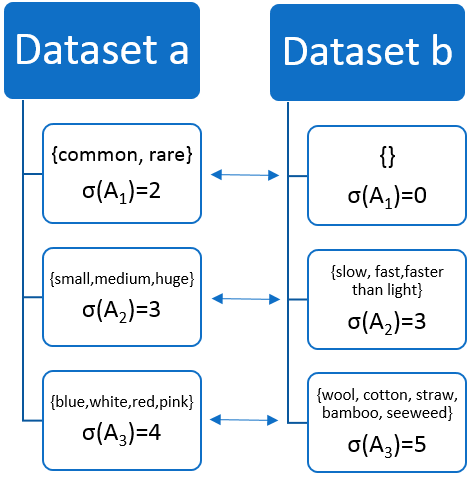
\includegraphics[width=7cm]{Images/example1.png}
		\centering
	\caption{Method one - attributes of datasets $a$ and $b$ were aligned according to their $\sigma$.}		\label{fig:example1}	
\end{figure} 
Now enumerate every aligned pair and sum up the differences between sigma values of each pair. The total distance is $|2-0|+|3-3|+|4-5|=2+0+1=3$.

We will use the same distance measure and the same datasets to demonstrate Algorithm \ref{algo:hungarianAlgorithm}. Let us define $IAttributeDistance$ function by building a distance matrix. The values of the distance matrix are in Table \ref{table:distance matrix}.
\begin{table}[htbp]
\caption{Distance matrix of the attributes of datasets $a$ and $b$. The matrix will serve as an input of the Hungarian algorithm.}
\label{table:distance matrix}
\centering
\begin{tabular}{ |c | c | c |c | }
  \hline
  & $a$ - $Att1$ & $a$ - $Att2$ & $a$ - $Att3$  \\
  \hline                       
  $b$ - $Att1$ & 1 & 2 & 3  \\
  $b$ - $Att2$ & 1 & 0 & 1  \\
  $b$ - $Att3$ ($\dummy$) & 4  & 3 & 2  \\  
  \hline  
\end{tabular}
\end{table}

By applying the Hungarian algorithm, we obtain the optimal alignment. The optimal alignment can be found in Table \ref{table:distancematrix2}.
\begin{table}
\caption{Results of application of the Hungarian algorithm. The optimal alignment is coloured.}
\label{table:distancematrix2}
\centering

\begin{tabular}{ |c | c | c |c | }
  \hline
  & $a$ - $Att1$ & $a$ - $Att2$ & $a$ - $Att3$  \\
  \hline                       
  $b$ - $Att1$ & \cellcolor{blue!25}1 & 2 & 3  \\
  $b$ - $Att2$ & 1 &\cellcolor{blue!25}0 & 1  \\
  $b$ - $Att3$ ($\dummy$) & 4  & 3 & \cellcolor{blue!25}2  \\
    \hline  
\end{tabular}
\end{table}

Algorithm \ref{algo:combinedAlignmentHungarian} adds selectors to the process. Imagine we have dataset $c$ defined in Table \ref{table:datasetc}. Suppose we have two selectors -- one for numerical and one for categorical attributes. New datasets emerge from the input dataset according to the selectors. In the case of dataset $c$ processed by the selectors, we will get two datasets. The first consisting solely of $Att1$ for the numerical selector and the second consisting solely of $Att2$ for the categorical selector.
This gives us a new assignment task for every selector. Such tasks are processed by attribute assignment algorithm (Algorithm \ref{algo:hungarianAlgorithm}) demonstrated above.
The algorithm finishes by weighting the inputs for each assignment result according to the given weights.

 \begin{table}[htbp]
	\caption{Possible values of dataset $c$.}
	\label{table:datasetc}
	\centering
	\begin{tabular}{ |c | c | c |c | }
		\hline
		$Att1$ & $Att2$  \\
		\hline                       
		1 &  Good \\
		4.5 &  Better \\
		3.7 &  Best \\
		5 &    \\
		2 &    \\
		\hline  
	\end{tabular}
\end{table} 

\subsubsection{Complexity Concerns}
The complexity of the assignment may be of a concern -- even though Hungarian algorithm is polynomial, its power can be too high. We do not expect this to be the case very often, since the model training usually takes quite a long time (for example, the problem of training the Neural Network with 3 hidden neurons is an NP-Complete problem \cite{neuralNetworkNPC}). Polynomial complexity for the recommendation is still just a negligible part of the whole process that can significantly reduce time of the training phase. Still, we would like to address the issue in case the complexity would be of concern. The complexities above are related to quality assessment of some algorithm. This is relevant when training new models, as the model assessment is part of the training. In the case of recommendation system being in production and new dataset arrives, the dataset distance is not needed for every pair of datasets but rather for the input and every other dataset. In case of the attribute assignment, the main burden lies in the Hungarian Algorithm.
%?Tarjan, Gabow - bounded
This can be mimicked by using approximate algorithms to solve the assignment problem:

\begin{definition}
Let $w(M)$ denote the weight of a matching in G, and $M^*$ a minimum-cost perfect matching in G. We call a perfect matching M \emph{$c$-approximate}, for $c \ge 1$, if $w(M) \le cw(M^*)$. 	
\end{definition}
In case the underlying matrix for assignment is a metric, we can use results of \cite{AgarwalApproximateBipartiteMatchingForMetric}. For any $\sigma > 0$, the authors present an algorithm that, in $$\mathcal{O}(n^{2+\sigma} \log n\log^2(1/\sigma))$$ time, computes a $\mathcal{O}(1/\sigma^\alpha)$-approximate matching of G, where $\alpha = \log_32 \approx 0.631$. 

\section{Theoretical Properties}
\label{section:theoreticalProperties}
In this section, we will explore interesting properties of the algorithms proposed in the previous section. We will show how the Assignments algorithm preserves metric properties, whether the same holds in opposite directions, and also we will be arguing about the best way of extending an attribute space with a $\dummy$ attribute.

Before we proceed to exploring the theoretical properties, we have to address a technicality. Consider the following situation. If the $\dummyinside$ is taken directly from the attribute space, it may theoretically happen that $\dummyinside$ will be compared to the equal attribute that was not dummy. However, to have at least a hope of obtaining a metric, we have to consider the case where the dataset with some attributes equal to $\dummyinside$ will be compared to almost the same dataset except that it will be missing the $\dummyinside$ attributes. The metric would require the distance between these datasets to be a non-zero. We have two ways to overcome this. We can also consider datasets equal if their attribute metadata are equal except any number of $\dummyinside$ like attributes. Another possibility is to modify the algorithm to distinguish between an artificial  $\dummyinside$ attribute and equal regular one and output some small non-negative number $\epsilon$ instead. At the same time, we would return $\epsilon + \attributeDistance(x,y)$ for non-matching input.
 In here we will use the former approach, as it will not clutter the text. However, we do not expect that this situation will happen often (or happen at all) as the attribute space will usually be of infinite size. 

\begin{theorem}
	\label{theorem:extendingOfAlignment}
	Let a, b be lists of attributes, f optimal alignment between a and b. Attribute distance measure $\attributeDistance$ is a metric on the extended space of attributes. Let $a' = a \cup \{\dummy_1\}$ and $b' = b \cup \{\dummy_2\}$, then $f'$ defined as 
	\begin{equation*}
	f'(x)=
	\begin{cases}
	f(x); \mbox{ if } x \in a, \\
	\dummy_2; \mbox{ otherwise}.
	\end{cases}
	\end{equation*}
	 is an optimal alignment between $a'$ and $b'$ with the same cost as f. This assignment extension is depicted in 
	 Figure \ref{fig:assignmentExtension}. 
	 \begin{figure}	
	 	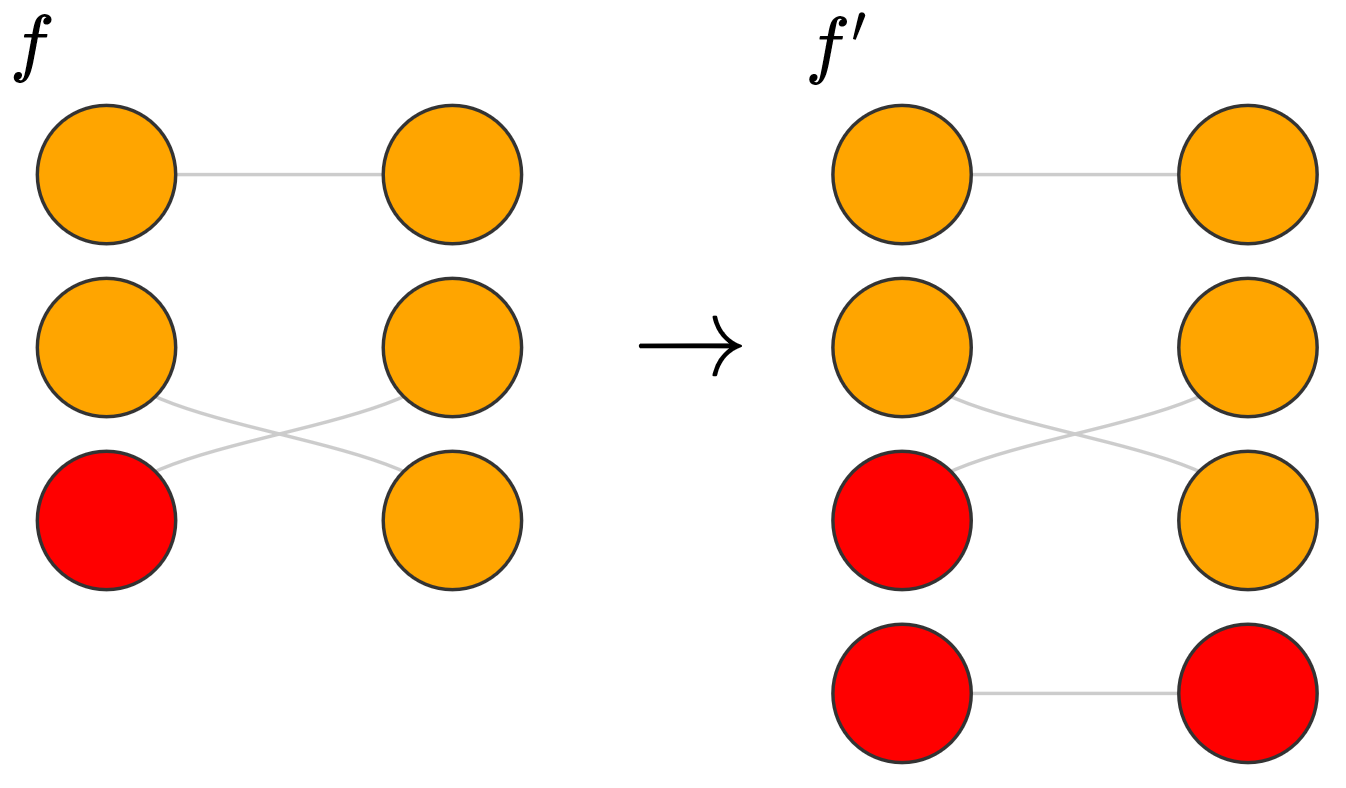
\includegraphics[width=7cm]{Images/assignmentExtension.png}
	 	\centering
	 	\caption{Extending optimal assignment by row of dummy attributes without changing the cost.}		\label{fig:assignmentExtension}	
	 \end{figure}
	\begin{proof}
		Suppose $f'$ is not an optimal assignment between $a'$ and $b'$ and some $f^*$ is. Observe that cost of $f'$ is the same as cost of $f$ because $\attributeDistance(\dummy_1, \dummy_2)=0$. Choose z so that $f^*(\dummy_1)=z$. If z is a dummy attribute, we can modify $f^*$ to $f'^*$ by swapping z and $\dummy_2$. Therefore $f'^*(\dummy_1)=\dummy_2$. As both $z$ and $\dummy_2$ are dummy attributes, this will not affect the cost of $f^*$. If $f'^*$ has lower cost than $f'$ (and thus consequently $f$), we can improve original $f,$ which is a contradiction. If it has the same cost then $f'$ must have been optimal which is also the contradiction. 
		
		The remaining case is that z is not dummy. Let k be $f^{*-1}(\dummy_2)$. Modify $f^*$ as follows:
		\begin{equation*}
		f'^*(x)=
		\begin{cases}
		z; \mbox{ if } x = k, \\
		\dummy_2; \mbox{ if } x = \dummy_1, \\
		f^*(x); \mbox{ otherwise}.
		\end{cases}
		\end{equation*}
		Let us examine cost of $f'^*$. We want to prove that this modification of $f^*$ to $f'^*$ did not increase the cost. As everything is the same except $\dummy_1$ and $k$, we need to investigate only those. We want to prove that $$\attributeDistance(k,z) + \attributeDistance(\dummy_1, \dummy_2) \le \attributeDistance(k,\dummy_2) + \attributeDistance(\dummy_1, z).$$
		Using the coincidence axiom the above is equivalent to
		$$\attributeDistance(k,z) \le \attributeDistance(k,\dummy_2) + \attributeDistance(\dummy_1, z)$$
		as $\attributeDistance(\dummy_1, \dummy_2)=0.$ This is of course true because it is an instance of triangle inequality.
	
 Now we can make the same argument we did with the z being a dummy attribute: If $f'^*$ has lower cost than $f'$ (and thus consequently $f$), we can improve original $f,$ which is a contradiction. If it has the same cost then $f'$ must have been optimal, which is also the contradiction. In all cases, $f'$ must have been optimal alignment.
	\end{proof}
\end{theorem}
By applying this theorem multiple times, we can add an arbitrary number of $\dummy$ attributes without changing the optimality of alignment.
\begin{theorem}
	\label{theorem:metricPreservation}
	Let a, b are list of attributes, $\attributeDistance$ is a metric on the extended space of attributes. Then Algorithm \ref{algo:attributeAlignmentHungarian} preserves all metric axioms and resulting distance $\globalDistance$ on the dataset space is a metric.
	\begin{proof} We will split the proof according to the different metric axioms.
	\begin{enumerate}
		\item We will begin with proving the non-negativity axiom. Since $\attributeDistance$ is a metric, it satisfies non negativity axiom. The cost of the minimal assignment must be non-negative as well.
		\item For the coincidence axiom we have to prove both direction of the equivalence:
		 \begin{itemize}
			\item $\Rightarrow:$ If $\globalDistance(x,y)=0$, the cost of minimal assignment was $0$. As $\attributeDistance$ satisfies non-negativity, it must be the case that all attributes were equal since $\attributeDistance$ also satisfies coincidence axiom. As all attributes were equal, the $x$ and $y$ must also be equal (up to permutation).
			\item $\Leftarrow:$ If $x=y$, all attributes must be equal (up to a permutation). Optimal solution is for every attribute assign the equal attribute. As $\attributeDistance$ satisfies coincidence and non-negativity, this optimal solution cost is 0.		
		\end{itemize}
		\item The proof of the symmetry axiom is as follows: given two datasets $a$ and $b$,
		the $a$ and $b$ are either of the same cardinality or the dataset with fewer attributes is extended by the appropriate number of  $\dummy$ attributes, so the cardinalities of the datasets match. This is done regardless of the order of the arguments. Therefore, for the rest of this part, we can assume that the dataset have the same number of attributes. Hungarian algorithm would find an optimal alignment $f$ -- a bijection from $a$ to $b$. If we would switch the arguments, algorithm would find the optimal bijection $g$ from $b$ to $a$.
		However, in both cases the algorithm would optimize the same thing, therefore the $\text{cost}(f) = \text{cost}(g)$, which would be the output of the algorithms regardless of their order.
		\item The remaining axiom to prove is the triangle inequality axiom. Let $x,y$ and $z$ be arbitrary datasets, $\attributeDistance$ metric on the attribute space and $\globalDistance$ dataset distance measure produced by the algorithm. We want to prove that $\globalDistance(x,y)\le \globalDistance(x,z) + \globalDistance(z,y).$ The algorithm would produce optimal assignments $f,g$ and $h$ between $x',y'$, $x,z$ and $z, y$ respectively. We can reformulate our goal to proving that  $\text{cost}(f) \le \text{cost}(g) +  \text{cost}(h).$ If the cardinality of the datasets would not match the corresponding amount of $\dummy$ attributes would be added to the datasets for the sake of the assignments. Now we will take maximum cardinality of the domains of the assignments:  $$max_{card}=\max(\mathbf{card}(\text{domain}(f),\mathbf{card}(\text{domain}(g),\mathbf{card}(\text{domain}(h)).$$
		
		We will now extend the datasets by adding extra $\dummy$ attributes so the number of attributes matches the $max_{card}.$ We get datasets $x', y'$ and $z'$.
		Corresponding new optimal assignments would be $f',g'$ and $h'$. We will argue that we did not change the costs of the assignments. If needed, algorithm would first add the $\dummy$ attributes to get the original assignments. If the domain does not match the $max_{card}$ we could use Theorem \ref{theorem:extendingOfAlignment}. With its help we could add the desired amount of $\dummy$ attributes finally reaching to extended datasets and another optimal assignment with the same cost as the original one. Note that the following now holds: $$\mathbf{card}(\text{domain}(f')=\mathbf{card}(\text{domain}(g')=\mathbf{card}(\text{domain}(h')).$$
		
		We proceed with creating the suboptimal assignment $f^\circ$ from $\text{domain}(f')$ to $\text{range}(f')$ by function composition of $g'$ and $h'$ -- $f^\circ=h'\circ g'$. We can do that as $\text{domain}(f')=\text{domain}(g')$ and $\text{range}(f')=\text{range}(h')$. As $f'$ is optimal we get 
		$$\text{cost}(f)=\text{cost}(f') \le \text{cost}(f^\circ)=
		\sum_{i=1}^{\text{len}(x')}\attributeDistance(x[i],f^\circ(x[i])).$$ 
		According to the fact that $\attributeDistance$ satisfies triangle inequality and the fact that $f^\circ=h'\circ g'$ we get
		$$\sum_{i=1}^{\text{len}(x')}\attributeDistance(x[i],f^\circ (x[i])) \le 
		\sum_{i=1}^{\text{len}(x')}(\attributeDistance(x[i],g'(x[i]))+ \attributeDistance(g'(x[i]),h'(g'(x[i])))).$$
		As $\text{range}(g')=\text{domain}(h')$ and every assignment function is a bijection, summing over elements of $x'$ is the same as summing over the permutation of elements of $x'$ given by assignments, we can conclude the proof:
		\begin{align*}
		\sum_{i=1}^{\text{len}(x')}(\attributeDistance(x[i],g'(x[i]))+ \attributeDistance(g'(x[i]),h'(g'(x[i]))))&=\text{cost}(g')+\text{cost}(h') \\
		& =\text{cost}(g)+\text{cost}(h).
		\end{align*}			 
		The whole proof of the triangle inequality is illustrated in Figure \ref{fig:metricPreservation}. 
		\begin{figure}	
			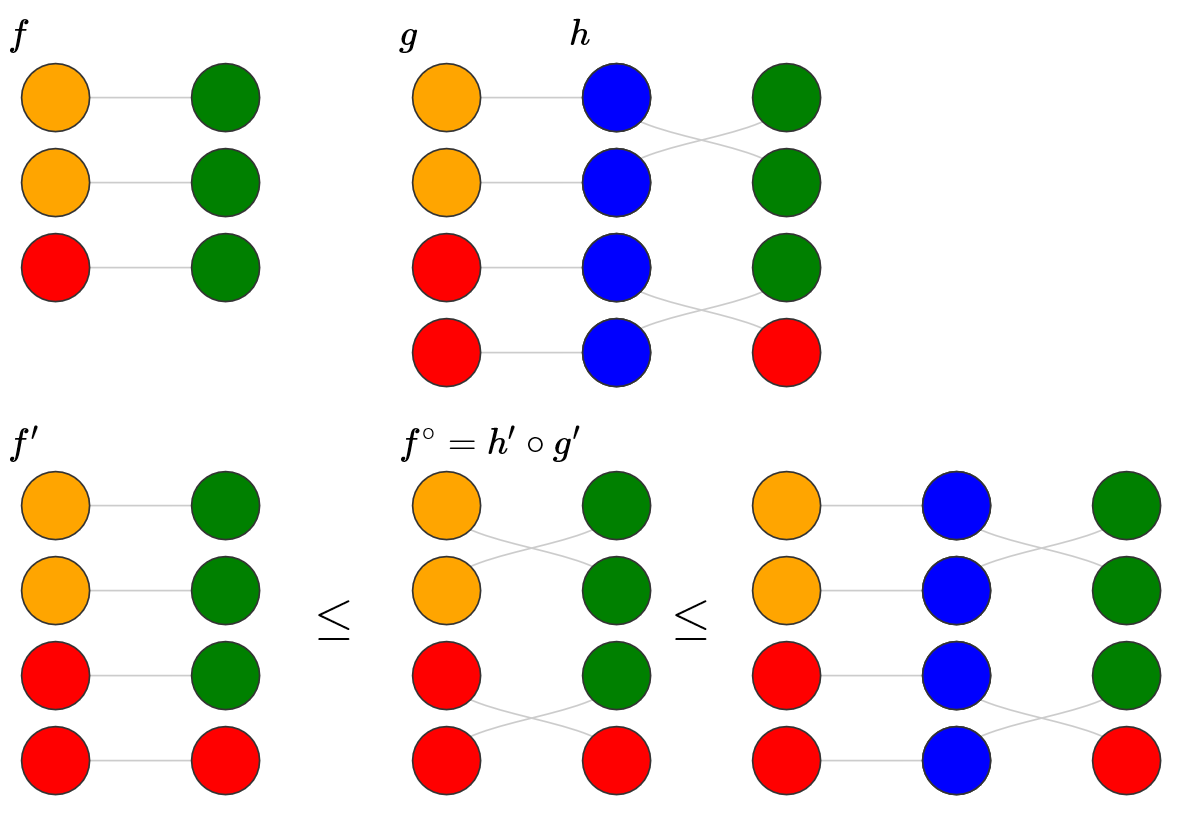
\includegraphics[width=14cm]{Images/metricPreservation.png}
			\centering
			\caption{Proof of Theorem \ref{theorem:metricPreservation} -- metric axiom 4 is preserved. Alignment $f$ is extended and then reshuffled so the triangle inequality can be applied. Yellow nodes are original attributes of dataset $x$, green nodes are attributes of dataset $y$ and blue of dataset $z$. Red nodes are $\dummy$ attributes used for extending the datasets so the corresponding assignments are of the same cardinality.}	
			\label{fig:metricPreservation}	
		\end{figure}
	\end{enumerate} 	
	As all metric axioms are proven, we can conclude the proof.	
	\end{proof}
\end{theorem}

The previous theorem also holds for Algorithm \ref{algo:combinedAlignmentHungarian}:
\begin{corollary}
		\label{corollary:metricPreservation}
		Let a, b are lists of attributes, $\{\attributeDistance_1, \dots, \attributeDistance_n \}$ are metrics on the extended space of attributes, $\{s_1, \dots, s_n\}$ are selectors, $\{w_1, \dots, w_n\}$ are positive weights of each selector. Then Algorithm \ref{algo:combinedAlignmentHungarian} preserves all metric axioms and resulting distance on the dataset space is a metric.	
	\begin{proof}
		Follows from the previous theorem and the fact that sum of metrics with positive weights is also a metric (Corollary \ref{corollary:weightedMetricAddition}).
	\end{proof}
\end{corollary}

It may be interesting to see how to extend attribute space by an artificial $\dummyoutside$ attribute. A following theorem gives us some clue: 
\begin{theorem}
	\label{theorem:dummyConstantMinimalDistance}
		Let $\attributeDistance'$ be a metric on a non-empty attribute space $\mathbb{A}$.	Let $\attributeDistance$ be a distance derived from $\attributeDistance'$ by extending  $\mathbb{A}$ by artificial $\dummyoutside$ attribute. We set the $\attributeDistance(\dummyoutside, x)$ and $\attributeDistance(x, \dummyoutside)$ to some constant $k$ $\forall x \in \mathbb{A}$. Finally, we set $\attributeDistance(\dummyoutside, \dummyoutside)=0.$ Let $\attributeDistance_{max}=\max_{x,y \in \mathbb{A}}\attributeDistance(x,y).$ If $\attributeDistance$ is a metric on the extended attribute space then $0 < k$ and $\frac{\attributeDistance_{max}}{2} \le k$.	
	\begin{proof}
		If $k < 0$ then $\attributeDistance(\dummyoutside, x)<0$, which would contradict non-negativity. If $k = 0$ then $\attributeDistance(\dummyoutside, x)=0$ and for every $x \in \mathbb{A}$ is $x \ne \dummyoutside$, which contradicts coincidence axiom.   
	The idea of the remaining part is as follows: we cannot short-cut our way when going on the longest way in the space by going through $\dummyoutside$ attribute which has the constant distance from every other point in the space -- this is depicted in Figure \ref{fig:constDummyTheorem}. 
	\begin{figure}	
		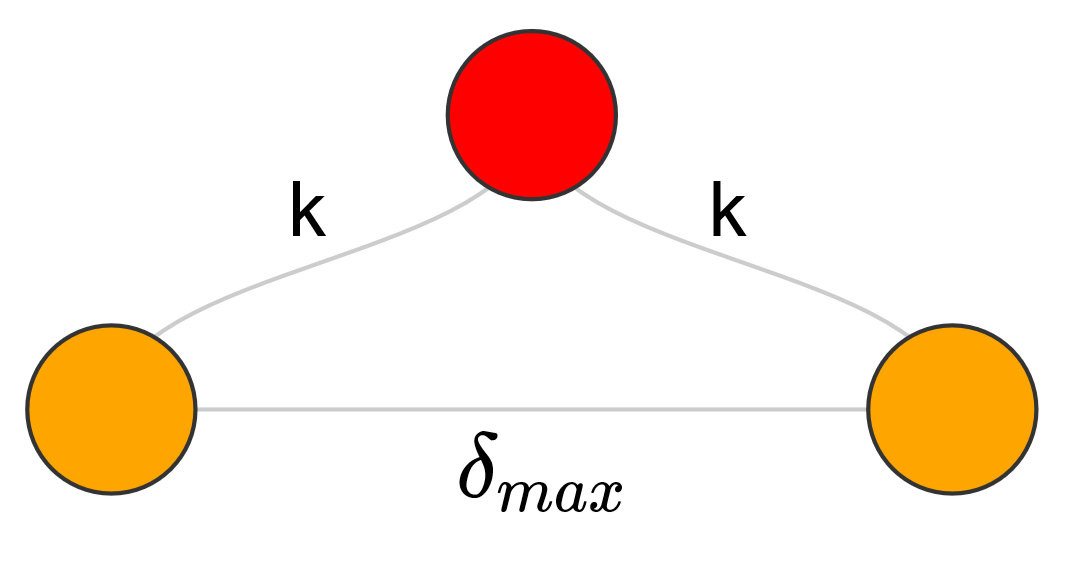
\includegraphics[width=7cm]{Images/constDummyTheorem.png}
		\centering
		\caption{Part of proof of Theorem \ref{theorem:dummyConstantMinimalDistance}. Constant $k$ representing a distance between a regular and an artificial  $\dummyoutside$ attribute  needs to be big enough in order not to create the shortcut between the most distant points.}	
		\label{fig:constDummyTheorem}	
	\end{figure}
	Find $x_0, y_0$ so that $\attributeDistance(x_0,y_0)=\attributeDistance_{max}$. From triangle inequality we get $ \forall x,y \in \mathbb{A}: \attributeDistance(x,y) \le \attributeDistance(x, \dummyoutside) + \attributeDistance(\dummyoutside, y)$. All the more true that $\attributeDistance(x_0,y_0) \le \attributeDistance(x_0, \dummyoutside) + \attributeDistance(\dummyoutside, y_0)$. As $\forall z \in \mathbb{A}:  \attributeDistance(\dummyoutside, z) = \attributeDistance(z, \dummyoutside) = k$ we get $\attributeDistance_{max} \le 2k$ which is equivalent to $\frac{\attributeDistance{max}}{2} \le k$.	
	\end{proof}
\end{theorem}
If we want to have metric attribute distance, and at the same time, a constant distance from artificial $\dummyoutside$ attributes, we have to choose this constant from quite large values. Doing this can create unwanted side affects. The penalty for adding $\dummyoutside$ attributes can become the most significant part of the distance, especially if the number of attributes varies by large amounts. It can be argued that if some attributes are not very relevant for the prediction of the target (for example attributes with low entropy), the two datasets should not differ too much if one dataset is missing such not very relevant attributes. Furthermore, in some cases it may be impossible to compute $\delta_{max}$ or to learn the value in advance. 

We get no such problems if we use the element of the attribute space itself, if we already made sure that the attribute distance is a metric. Using the $\dummyinside$ attribute from the space will not break the metric axioms (if the attribute distance $\attributeDistance$ is a metric).

Theorem \ref{theorem:metricPreservation} is also valid in the opposite direction, as shown in the following theorem.
\begin{theorem}
	\label{theorem:metricRestoration}
	Let a, b are list of attributes, $\attributeDistance$ is a distance between attributes. If $\globalDistance$ is a distance over dataset space produced by Algorithm \ref{algo:attributeAlignmentHungarian} and $\globalDistance$ is a metric on the dataset space, then $\attributeDistance$ is a metric on the extended attribute space $\mathbb{A}$.
	\begin{proof} Again, we will split the proof according to the different metric axioms.
		\begin{enumerate}
			\item We will begin with proving the non-negativity axiom. 	For the sake of contradiction, let us suppose that $\attributeDistance$ does not satisfy non-negativity axiom. It must be the case that $\exists x,y \in \mathbb{A}$ so $\attributeDistance(x,y) < 0$. We define datasets $X$ and $Y$ consisting solely of $x$ and $y$ respectively. There is only a single assignment $f$ available -- mapping $x$ to $y$ and is therefore optimal. Algorithm \ref{algo:attributeAlignmentHungarian} will output the $\text{cost}(f)$:  $\globalDistance(X,Y)\sum_{i=1}^{1}\attributeDistance(X[i],f(X[i]))=\attributeDistance(x,y)$. We get a contradiction as $\globalDistance(X,Y) \ge 0$ and $\attributeDistance(x,y) < 0$.
			\item For the coincidence axiom we have to prove both direction of the equivalence:
			\begin{itemize}
				\item $\Rightarrow:$  If $\attributeDistance(x,y)=0 \land x \ne y$, we define datasets $X$ and $Y$ consisting solely of x and y respectively. $X \ne Y$ and as $\globalDistance$ is a metric we get $\globalDistance(X,Y) > 0$. As $\mathbf{card} (X) = \mathbf{card} (Y)=1$ there is only a single assignment $f$ available and must be the optimal alignment returned by Algorithm \ref{algo:hungarianAlgorithm}. The cost outputted by Algorithm \ref{algo:attributeAlignmentHungarian} is $\globalDistance(X,Y)\sum_{i=1}^{1}\attributeDistance(X[i],f(X[i]))=\attributeDistance(x,y)=0,$ which is a contradiction.
				\item $\Leftarrow:$  If $x=y \land \attributeDistance(x,y)>0$  we define datasets $X$ and $Y$ consisting solely of x. $X = Y$ and as $\globalDistance$ is a metric we get $\globalDistance(X,Y) = 0$. As $\mathbf{card} (X) = \mathbf{card} (Y)=1$ there is only a single assignment $f$ available and must be the optimal alignment used by Algorithm \ref{algo:attributeAlignmentHungarian}. The cost outputted by the algorithm is $\globalDistance(X,Y)\sum_{i=1}^{1}\attributeDistance(X[i],f(X[i]))=\attributeDistance(x,y)>0,$ which is a contradiction.		
			\end{itemize}
			\item The proof ot the symmetry axiom is as follows. For the sake of contradiction, let us assume that $\attributeDistance$ does not satisfy symmetry axiom. It must be the case that $\exists x,y \in \mathbb{A}$ so $\attributeDistance(x,y) \ne \attributeDistance(y,x)$. We will define datasets $X$ and $Y$ consisting solely of $x$ and $y$ respectively. There is only a single assignment $f$ from $X$ to $Y$ available -- mapping $x$ to $y$ and is therefore optimal. Similarly, there is only a single assignment $g$ from $Y$ to $X$ available -- mapping $y$ to $x$ and is therefore optimal. Algorithm \ref{algo:attributeAlignmentHungarian} will output the $\text{cost}(f)$:  
			$$\globalDistance(X,Y)\sum_{i=1}^{1}\attributeDistance(X[i],f(X[i]))=\attributeDistance(x,y).$$
			The $\text{cost}(g)$ is computed analogically: $$\globalDistance(Y,X)\sum_{i=1}^{1}\attributeDistance(Y[i],g(Y[i]))=\attributeDistance(y,x).$$ 
			We get a contradiction. As $\globalDistance$ satisfies symmetry axiom we get $\globalDistance(X,Y) = \globalDistance(Y,X)$. However, at the same time we have $\globalDistance(X,Y) \ne \globalDistance(Y,X)$ from assumptions.
			\item The remaining axiom to prove is the triangle inequality axiom. For the sake of contradiction, let us suppose that $\attributeDistance$ does not satisfy triangle inequality. It must be the case that $\exists x,y,z \in \mathbb{A}$ so $\attributeDistance(x,y) > \attributeDistance(x,z)+\attributeDistance(z,x)$. We will  define datasets $X$, $Y$ and $Z$ consisting solely of $x$,$y$ and $z$ respectively. There is only a single assignment $f$ from $X$ to $Y$ available -- mapping $x$ to $y$ and is therefore optimal. Similarly, there is only a single assignment $g$ from $X$ to $Z$ available and only a single assignment $h$ from $Z$ to $Y$ -- both are also optimal. Algorithm \ref{algo:attributeAlignmentHungarian} will output the $\text{cost}(f)$:
			$$\globalDistance(X,Y)\sum_{i=1}^{1}\attributeDistance(X[i],f(X[i]))=\attributeDistance(x,y).$$
			Again, the $\text{cost}(g)$ and $\text{cost}(h)$ are computed analogically:
			\begin{equation*}
			\globalDistance(X,Z)\sum_{i=1}^{1}\attributeDistance(X[i],g(X[i]))=\attributeDistance(x,z),
			\end{equation*}
			\begin{equation*}
			\globalDistance(Z,Y)\sum_{i=1}^{1}\attributeDistance(Z[i],h(Z[i]))=\attributeDistance(z,y).
			\end{equation*}
			 As $\globalDistance$ satisfies triangle inequality we have $\globalDistance(X,Y) \le \globalDistance(X,Z)+\globalDistance(Z,Y).$ At the same time we have $\globalDistance(X,Y) > \globalDistance(X,Z)+\globalDistance(Z,Y)$ from assumptions, which is a contradiction.
		\end{enumerate}
			As all metric axioms are proven, we can conclude the proof.	
		\end{proof}	
\end{theorem}

Similar theorem holds for Algorithm \ref{algo:combinedAlignmentHungarian} with addition that all selectors must be distinct:
\begin{corollary}
		\label{corollary:metricRestoration}
		Let a, b are list of attributes, $\{\attributeDistance_1, \dots, \attributeDistance_n\}$ are the distances on the extended space of attributes, $[s_1, \dots, s_n]$ are selectors, $[w_1, \dots, w_n]$ are weights of each selector. If $\forall k,j \in \left\{1, \dots, n\right\}, \forall \mathbb{A'} \subseteq \mathbb{A}:s_k(\mathbb{A'})\bigcap s_j(\mathbb{A'})= \emptyset$ and distance $\globalDistance$ produced by Algorithm \ref{algo:combinedAlignmentHungarian} is a metric on the dataset space then $\{\attributeDistance_1, \dots, \attributeDistance_n\}$ are metrics on the extended attribute space defined by the corresponding selector.	
	\begin{proof}
		We can prove the corollary by following the proof of the previous theorem. When creating dataset of a single element, we now do this for every $\attributeDistance_i$ that does not satisfy axiom in question. As selectors are distinct, other selectors will return $\emptyset$ from single element datasets and therefore will output 0 for corresponding selector distance, as the resulting distance is the sum over all attributes returned by the selector.
	\end{proof}
\end{corollary}
It is intuitive to have each selector distinct, if we think of a selector in the sense we have introduced them: selector selects specific attributes (e.g. categorical or numerical) so more fine grained distance functions can be applied. In this sense the selectors will be distinct as the subset of categorical attributes is clearly disjunct to subset of numerical attributes.

We can wonder whether Corollary \ref{corollary:metricRestoration} holds even without the constraint for distinct selectors. 
\begin{observation}
The requirement for distinct selectors is an essential part of Corollary \ref{corollary:metricRestoration}. 
\begin{proof}
	We will show a counterexample: let attribute space be the set of two elements: $\mathbb{A}={a_1, a_2}$.
	Let $s_1,s_2$ be two selectors defined as $s_1(\mathbb{X})=s_2(\mathbb{X})=\mathbb{X}$. Let $\attributeDistance_1$ be a metric and $\attributeDistance_2$ be a distance function defined as $\attributeDistance_2(x,y)=-0.1\attributeDistance_1(x,y)$. $\attributeDistance_2$ is not a metric on the attribute space as it violates non-negativity -- $\attributeDistance_2(a_1, a_2) = -0.1\attributeDistance_1(a_1, a_2) < 0$. It still satisfies symmetry and coincidence though. We can combine $\attributeDistance_1$ and $\attributeDistance_2$ to form $\attributeDistance_3$: $\attributeDistance_3(x,y) = \attributeDistance_1(x,y)+\attributeDistance_2(x,y)=0.9\attributeDistance(x,y)$. $\globalDistance$ induced by $\attributeDistance_1$, $\attributeDistance_2$, and $s_1 = s_2$ is the same as $\globalDistance'$ induced by $\attributeDistance_3$. $\attributeDistance_3$ is a metric on the attribute space according to Theorem \ref{theorem:metricrescaling} as it is positively rescaled $\attributeDistance_1$. Therefore, it does not matter if we use the combination of $\attributeDistance_1,\attributeDistance_2$ or just $\attributeDistance_3$ alone. Resulting $\globalDistance$ is a metric on the dataset space according to Theorem \ref{theorem:metricPreservation} even-though $\attributeDistance_2$ is not a metric on the dataset space.
\end{proof}
\end{observation}

Theorems \ref{theorem:metricPreservation}, \ref{theorem:metricRestoration} and Corollaries \ref{corollary:metricPreservation} and  \ref{corollary:metricRestoration} are useful as they state that if we can get a metric on the attribute or dataset space, we get other metric on the other space for free when using attribute aligning. During training, we could define a function measuring metric similarity on the attribute or dataset samples. As the samples would usually be just small finite subsets of attribute or datasets space, we could be wondering whether by optimizing metric on some dataset or attribute subset, we would get also metric on the other subset as Theorems \ref{theorem:metricPreservation}, \ref{theorem:metricRestoration} and Corollaries \ref{corollary:metricPreservation}, \ref{corollary:metricRestoration} are valid only for the whole spaces. We will try to formalize this motion:

\begin{definition}
\label{definition:supportedDatasets}
Let $\mathbb{A}$ be attribute space, let $A$ be the subset of $\mathbb{A}$. Let $\mathbb{D}$ be a dataset space. Then we will denote dataset subspace $D$ as \emph{supported} by attribute subspace $A$ if $D \subseteq \mathbb{D}$ and if $\forall d \in D,\forall att \in d:att \in A$. 
\end{definition} 
In other words, datasets in $D$ are only composed of elements in $A$. This definition allow us to investigate metric properties in just the subset of attribute spaces and conclude properties in supported subspaces of datasets (like training and testing subset) and vice-versa.

\begin{definition}
Let $\mathbb{A}$ be attribute space, let $\mathbb{D}$ be a dataset space and $D$ its subset. We will call the subset $A$ of $\mathbb{A}$ as the \emph{source} of $D$ if $\forall att \in \mathbb{A}: att \in A \iff \exists d \in D: att \in d$. 
\end{definition} 
In other words, elements of $A$ are just enough in order to create all elements in $D$. Similarly to the remark to Definition \ref{definition:supportedDatasets}, we can use this definition to reason about whether properties that are valid for some distance function on some set of datasets are also valid for the attribute source of these datasets.

If we optimize metric on subset of attributes, we also get metric on all datasets that can be combined by this subset of attributes when using Algorithm \ref{algo:attributeAlignmentHungarian}:
\begin{theorem}
\label{theorem:metricPreservationSuportedSpaces}
Let $\mathbb{A}$ be extended space of attributes and $A$ its extended subset, $\attributeDistance$ is a metric on $A$, $\mathbb{D}$ space of datasets. Then $\forall D \subseteq \mathbb{D}$, $D$ supported by $A$: Algorithm \ref{algo:attributeAlignmentHungarian} preserves all metric axioms and resulting distance $\globalDistance$ on the $D$ is a metric.
	\begin{proof}
	From following the proof of Theorem \ref{theorem:metricPreservation} as the proof does not require elements outside of $D$ or $A$ and we can replace the whole $\mathbb{D}$ by $D$ and $\mathbb{A}$ by $A$.
	\end{proof}
\end{theorem}
Intuitively, the same works for Algorithm \ref{algo:combinedAlignmentHungarian}.

This enables us to define our algorithms in such a way, that if we can create a metric on all the attributes in the training and testing samples, we can also guarantee the resulting metric on all supported subsets of the dataset space. The training and testing datasets must be among them, as they are supported by the testing and training attributes.

Note that Theorem \ref{theorem:metricPreservationSuportedSpaces} is valid because there is nothing in the proof of Theorem~\ref{theorem:metricPreservation} that would require elements (datasets) outside of the subset $D$ and $A$. As for the other direction,  when observing the proof of Theorem \ref{theorem:metricRestoration}, we use the trick that we artificially create datasets with a single element. However, such datasets can be outside of $D$. We can then wonder whether Theorem \ref{theorem:metricPreservationSuportedSpaces} is valid also in the other direction considering  Algorithm \ref{algo:attributeAlignmentHungarian}. It is not according to Observation~\ref{theorem:metricNonRestorationSupportedSpaces}.

\begin{observation}
	\label{theorem:metricNonRestorationSupportedSpaces}
	Let $\mathbb{A}$ be space of attributes and $\mathbb{D}$ space of datasets. Let $D$ be a subset of $\mathbb{D}$ and $\globalDistance$ a metric on $D$. Let $A$ be the source of $D$ and $\attributeDistance$ be a distance measure on $A$, such that Algorithm \ref{algo:attributeAlignmentHungarian} induces $\globalDistance$ using $\attributeDistance$. Then $\attributeDistance$ is not necessarily a metric on $A$.
	\begin{proof}
	We will show a counterexample.
	Let $\mathbb{A}$ be the space of attributes, $D$ be the subspace of datasets  consisting of single dataset $d=\left\lbrace a_1, a_2, a_3 \right\rbrace$. Let $A=\left\lbrace a_1, a_2, a_3 \right\rbrace \subseteq \mathbb{A}$ the source of $D$. Let $\globalDistance$ be a metric on  $D$. Since $D$ consists of only one element, in order $d$ to be a metric all we need to do is set $\globalDistance(d,d)=0$. Let $\attributeDistance$ be attribute distance function on $A$. We will show that even though $\globalDistance$ is a metric, $\attributeDistance$ does not have necessarily to be a metric. We can define $\attributeDistance$ as shown in Table \ref{table:supportAttributeCounterexample}. As there are some negative values, the attribute distance $\attributeDistance$ is not a metric.
	\begin{table}
		\caption{Counterexample that metric on some subspace of datasets does not imply metric on its source attribute subspace}
		\label{table:supportAttributeCounterexample}
		\centering
		\begin{tabular}{ |c | c | c |c | }
			\hline
			& $a_1$ & $a_2$ & $a_3$  \\
			\hline                       
			$a_1$ & \cellcolor{blue!25} 0 & 50 & 50  \\
			$a_2$ & 50 &\cellcolor{blue!25}-5 & 50  \\
			$a_3$ & 50  & 50 & \cellcolor{blue!25}5  \\
			\hline  
		\end{tabular}
	\end{table}
	The optimal alignment $f$ between $d$ and $d$ is coloured and is defined as $f(a_i)=a_i$.
	The $\text{cost}(f)=\attributeDistance(a_1,a_1)+\attributeDistance(a_2,a_2)+\attributeDistance(a_3,a_3)=0+5-5=0=\globalDistance(d,d)$.
	\end{proof}
\end{observation}

Same counterexample can be found when using Algorithm \ref{algo:combinedAlignmentHungarian} as this algorithm is a generalization of Algorithm \ref{algo:attributeAlignmentHungarian}, therefore the same argument can be applied. 
This implies that we cannot guarantee metric on the subspace of attributes appearing in the training and testing datasets even if we can guarantee resulting distance to be a metric on the training and testing dataset subspace.

Another argument favouring a metric for the attributes is that specialized algorithms can be used for the assignment such as \cite{AgarwalApproximateBipartiteMatchingForMetric}.

\section{Distance Using Attribute Metadata}
In Section \ref{section:distanceUsingGlobalMetadata}, we discussed distance based on a vector of global metafeatures. We can analogically define a distance on the attribute space or subspace defined by some selector. This can be then the $IAttributeDistance$ input for Algorithms \ref{algo:attributeAlignmentHungarian} and \ref{algo:combinedAlignmentHungarian}.

\IncMargin{1em}
\begin{algorithm}
\SetKwInOut{Input}{input}
\SetKwInOut{Output}{output}
\tcp{Pseudocode for measuring distance between attribute treating attributes as real valued vector.}
\Input{$\sigma$ $\leftarrow$ Vector distance measure}
\Input{$x \leftarrow$ First attribute}
\Input{$y \leftarrow$ Second attribute}
\Output{Distance between two attributes}
\BlankLine
$\text{vector}_x \leftarrow x_{\text{attribute\_metafeatures}}$\;
$\text{vector}_y \leftarrow y_\text{attribute\_metafeatures}$\;
distance $\leftarrow \sigma(\text{vector}_x,\text{vector}_y)$\;
\Return $distance$\;
\caption{Vectorized Attribute Distance: $IAttributeDistance$}\label{algo:basicAttributeDistance}
\end{algorithm}\DecMargin{1em}
\emph{Attribute\_metafeatures} is a property returning real value vector of attribute metafeatures for a given attribute.
This property does not have to be necessarily defined on the whole attribute space. For example, in the case of Algorithm \ref{algo:combinedAlignmentHungarian} it must be defined only on the subspace of attributes defined by the corresponding selector, e.g. it can return vector of features specific for numerical attributes in the case of numerical selector.


Again, note that both variables $\text{vector}_x, \text{vector}_y$ are real valued vectors of the same length $n$. This allows us to use any metric defined on $\mathbb{R}^n$ including all the metrics based on $p$-norms (Theorem \ref{theorem:pnormisnorm}) and their weighted counterparts (Theorem~\ref{theorem:weightedpnormisnorm}) and the resulting attribute measure will also be a metric. Using such metric in Algorithms \ref{algo:attributeAlignmentHungarian} and \ref{algo:combinedAlignmentHungarian} will preserve the metric and the resulting dataset distance will be also a metric according to Theorems \ref{theorem:metricPreservation} and \ref{theorem:metricPreservationSuportedSpaces}, and Corollary \ref{corollary:metricPreservation} and its selector counterpart.

\section{Combining the Distances}
We have dedicated lots of effort to utilize extra information from the attributes. We have the whole workflow that builds the distance on the datasets from the attribute distance through aligning and selectors. In this section, we would like to address the fact that global attributes store useful information as well -- this was proven in the literature. Even though the attribute alignment was competitive to global dataset distances, it does not necessarily mean that we have to use them separately from each other. In fact, it could be useful to combine their powers to get even better distance measure between datasets. In order to achieve this we have proposed Algorithm \ref{algo:datasetDistanceCombination}.

\IncMargin{1em}
\begin{algorithm}
\SetKwInOut{Input}{input}
\SetKwInOut{Output}{output}
\tcp{Pseudocode for combining multiple dataset distance measure and producing their weighted combination.}
\Input{distances $\leftarrow$ List of dataset distance measures $\globalDistance$}
\Input{weights $\leftarrow$ List of weights}
\Input{$x$ $\leftarrow$ First dataset}
\Input{$y$ $\leftarrow$ Second dataset}
\Output{Distance between two datasets}
\BlankLine
distance $\leftarrow 0$\;
\For{\upshape $i$ in $\lbrace 1,\dots, \text{len(distances)} \rbrace$}{
distance $\leftarrow$ distance + weights[$i$]distances[$i$]$(x,y)$\;
}
\Return distance\;
\caption{Dataset Distance Aggregation: $IDatasetDistance$}\label{algo:datasetDistanceCombination}
\end{algorithm}\DecMargin{1em}

This algorithm takes list of dataset distance measures and weights their results.
If the underlying datasets measures are metric and weights are positive, the algorithm will also produces a metric on the datasets space according to the fact that weighted sum of metrics is also a metric, if the weights are positive (Corollary \ref{corollary:weightedMetricAddition}).
As usual, using the $partial$ application we can conform to the $IDatasetDistance$ interface, if we fix all the arguments except the last two.

\section{Normalization Based on the Number of Attributes}
When using Algorithms \ref{algo:attributeAlignmentMasterThesis}, \ref{algo:attributeAlignmentHungarian} and \ref{algo:combinedAlignmentHungarian}, after getting the total distance defined by the optimal alignment, we could think about normalizing this distance by the number of attributes. This would amend the algorithms. Algorithm \ref{algo:attributeAlignmentHungarian} would return $\frac{TotalDistance}{NumberOfAttributes}$ instead. Algorithm \ref{algo:combinedAlignmentHungarian} would do this amendment for each selector (and number of attributes would be based on the number of attributes selected by the selector). Such amendments would normalize this distance to a count independent on the attribute number. This may or may not be beneficial, but in this section we show that there are theoretical reasons against it.

There are two natural ways how to normalize by the number of attributes. Given two datasets $a$ and $b$ with the number of attributes $|a|$ and $|b|$, we can either divide the total distance by $\min(|a|,|b|)$ or by $\max(|a|,|b|)$.
We will start by exploring the latter case -- $\max(|a|,|b|)$. Without the normalization, if the underlying attribute distance is a metric, the metric preservation to the dataset distance is ensured by Theorem \ref{theorem:metricPreservation}. We will show that this is not necessary true if we do the normalization according to the $\max(|a|,|b|)$.

\begin{observation}
	Normalizing the distance by $\max(|a|,|b|)$ can violate metric axioms.
	\begin{proof}
		Let $\attributeDistance$ be a metric on the extended attribute space $\mathbb{A}$, $\dummy \in \mathbb{A}$, $a=\lbrace a_1 \rbrace,b= \lbrace b_1 \rbrace$ are datasets. Let us define the $\attributeDistance(a_1,b_1)$ as 1 and set $\attributeDistance(a_1,\dummy)=\attributeDistance(b_1,\dummy)=10$. The optimal alignment is the only one possible, $\max(|a|,|b|)$ is 1, therefore distance $\globalDistance$ returned by the normalized Algorithm \ref{algo:attributeAlignmentHungarian} is $\frac{1}{1}$. We will show that the triangle inequality does not have to be preserved. We will define dataset $z$ as $\lbrace a_1,\dummy \rbrace$. For the triangle inequality to hold, it must be the case that $\globalDistance(a,b) \le \globalDistance(a,z)+\globalDistance(z,b)$. Let us see what $\globalDistance(a,z)$ is. One $\dummy$ attribute will be added, as $\attributeDistance(\dummy,\dummy)=0$, we get optimal alignment of the cost of zero as it will align $a_1$ to $a_1$ and $\dummy$ to $\dummy$. The zero will be divided by  $\max(|a|,|z|)$ resulting in $\globalDistance(a,z)=0$. As for the $\globalDistance(z,b)$, one $\dummy$ attribute is again added to $b$,  the optimal alignment is either $a_1 \rightarrow b_1, \dummy \rightarrow \dummy$ or $a_1 \rightarrow \dummy, \dummy \rightarrow b_1$. The cost of the former is 1, the cost of the latter is $2 \times 10=20$ . Therefore, the former is optimal. As $\max(|b|,|z|)=2$ we get $\globalDistance(z,b)=1/2$.
		Finally we get $1=\globalDistance(a,b) \le \globalDistance(a,z)+\globalDistance(z,b)=1/2$ which is not valid and distance on the dataset space $\globalDistance$ is not a metric, as the triangle inequality was broken.
	\end{proof}
\end{observation}

The same holds for the former case -- $\min(|a|,|b|)$.

\begin{observation}
	Normalizing the distance by $\min(|a|,|b|)$ can violate metric axioms.
	\begin{proof}
		 Again, let $\attributeDistance$ be a metric on the extended attribute space $\mathbb{A}$, $\dummy \in \mathbb{A}$. But this time we define $a=\lbrace a_1, a_2 \rbrace, b= \lbrace b_1 \rbrace$. Let us define $\attributeDistance(a_1,b_1)=\attributeDistance(a_2,\dummy)=1$ and set $\attributeDistance(a_2,b_1)=10$. The optimal alignment is -- after adding one dummy attribute $\dummy$ to $b$ -- $a_1 \rightarrow b_1$ and $a_2 \rightarrow \dummy$. The cost of this alignment is 2 and as $\min(|a|,|b|)=1$ the resulting $\globalDistance(a,b)=2/1=1$. Again, we break the triangle inequality. We will define dataset $z$ as $\lbrace b_1,\dummy \rbrace$. For the triangle inequality to hold, it must be the case that $\globalDistance(a,b) \le \globalDistance(a,z)+\globalDistance(z,b)$. The $\globalDistance(a,z)$ is calculated according to the optimal alignment. As $z$ is the same as $b$ with one added $\dummy$ attribute, the optimal alignment must be the same as the optimal alignment from $a$ to $b$. The cost is therefore also 2. But this time $\min(|a|,|z|)=2$ and we get $\globalDistance(a,z)=2/2=1$. As for the $\globalDistance(z,b)$ we use the same argument -- $z$ is the same as $b$ with added $\dummy$. During the alignment, one $\dummy$ will be truly added to $b$ and consequently the cost of the optimal alignment will be zero. $\globalDistance(z,b)$ is therefore 0. Finally we get $2=\globalDistance(a,b) \le \globalDistance(a,z)+\globalDistance(z,b)=1$, which again breaks the triangle inequality and therefore $\globalDistance$ is not a metric.
	\end{proof}
\end{observation}

We have given the counterexamples for Algorithm \ref{algo:attributeAlignmentHungarian}, however the same is valid for Algorithm \ref{algo:combinedAlignmentHungarian}. As already stated in Section \ref{section:distanceUsingAttributes}, Algorithm \ref{algo:attributeAlignmentHungarian} is a special case of Algorithm  \ref{algo:combinedAlignmentHungarian} and every counterexample is therefore valid even for more generic algorithm.

According the theoretical results stated in this section, we will not use this normalization in the rest of the thesis as this modification could violate metric axioms of the resulting dataset distance.